%% LyX 2.1.4 created this file.  For more info, see http://www.lyx.org/.
%% Do not edit unless you really know what you are doing.
\documentclass[oneside,spanish,british]{book}
\usepackage{ae,aecompl}
\renewcommand{\sfdefault}{cmss}
\renewcommand{\familydefault}{\sfdefault}
\usepackage[T1]{fontenc}
\usepackage[latin9]{inputenc}
\setcounter{secnumdepth}{4}
\setcounter{tocdepth}{3}
\setlength{\parskip}{\medskipamount}
\setlength{\parindent}{0pt}
\usepackage{babel}
\addto\shorthandsspanish{\spanishdeactivate{~<>}}

\usepackage{array}
\usepackage{verbatim}
\usepackage{varioref}
\usepackage{float}
\usepackage{wrapfig}
\usepackage{fancybox}
\usepackage{calc}
\usepackage{textcomp}
\usepackage{url}
\usepackage{amstext}
\usepackage{graphicx}
\usepackage[unicode=true,pdfusetitle,
 bookmarks=true,bookmarksnumbered=false,bookmarksopen=false,
 breaklinks=false,pdfborder={0 0 0},backref=false,colorlinks=false]
 {hyperref}

\makeatletter

%%%%%%%%%%%%%%%%%%%%%%%%%%%%%% LyX specific LaTeX commands.
%% Because html converters don't know tabularnewline
\providecommand{\tabularnewline}{\\}

%%%%%%%%%%%%%%%%%%%%%%%%%%%%%% User specified LaTeX commands.
\usepackage{a4wide}
\usepackage{url}
\pagenumbering{roman}

\usepackage[T1]{fontenc}

\makeatother

\begin{document}

\title{{\huge{}Chronojump} Manual}


\author{http://www.chronojump.org\\
\\
Xavier de Blas Foix (2004-2013)\\
Xavier Padull�s Chando (2014-).\\
\\
English translation by: Helena Olsson.}

\maketitle
\pagebreak{}

\vspace*{17cm}


\noindent Licence of this document: Creative Commons Attribution-ShareAlike
3.0 Unported \url{http://creativecommons.org/licenses/by-sa/3.0/deed.en}\\
\\
Find the last version of this document in last version of Chronojump
software and here:

\noindent \url{http://www.chronojump.org/documents.html}

\thispagestyle{empty}

\noindent \rule[0.5ex]{1\linewidth}{1pt}

\frontmatter

\tableofcontents{}

\listoffigures


\listoftables


\mainmatter


\chapter{Introduction: Chronojump as a free software collaborator project
in sport science}

\emph{{[}Pending{]}}


\section{introduction}


\subsection{Instruments}


\subsection{Jump tests}


\subsubsection{Seargent test}


\subsubsection{Abalakov test}


\subsubsection{Bosco test}


\subsubsection{Specific jumps}


\subsection{Run tests}


\subsubsection{Simple runnings}


\subsubsection{Interval runnings}


\subsubsection{Agility circuits}


\subsection{Reaction time}


\subsection{Rhythms}


\subsection{Other tests}

\newpage{}


\part{Obtaining and configuring the software and the hardware}


\chapter{Obtaining the software and the hardware}

To use Chronojump technology is necessary: 
\begin{description}
\item [{Detection~device}] one or more contact platforms or photocells
or one encoder. 
\item [{Chronopic}] (chronometric device responsible to receive the changes
in the detection device) 
\item [{Chronojump}] management software. 
\item [{Computer}] with Windows, OSX or Linux operating system connected
to chronometer Chronopic and executing the software Chronojump. 
\end{description}

\section{Chronojump software installation}

Chronojump is free software which works with Windows, OSX and Linux
operating systems. To be download at the web page \url{http://chronojump.org/software.html}.

For more information consult the frequent asked questions of the software
(FAQ) \url{http://chronojump.org/faq_software.html}.


\section{Acquisition and construction of the detection device}

If you like to buy measuring device please check online shop at the
web page \url{http://www.chronojump.org/hardware_store.html}

To build your own contact platform or photoelectric cell, consult
at the hardware section at the web page \url{http://chronojump.org/documents.html}


\section{\label{sub:Construcci=0000F3n-y-obtenci=0000F3n-chronopic}Acquisition
and construction of the Chronopic chronometer}

If you like to buy the Chronopic chronometer, please check online
shop at the web page: \url{http://chronojump.org/pricing.htm} 

If you want to build your own Chronopic please check the section Hardware
at the web page: \url{http://chronojump.org/documents.html#hardware}

For more information consult the frequent questions of the software
(FAQ) \url{http://www.chronojump.org/faq_hardware.html}


\chapter{\label{par:Chronopic:-concepto-y-configuracion} Configuring Chronopic}

Chronopic is an integrated circuit used by Chronojump to detect the
test done at the detection device. To obtain the Chronopic please
check section \ref{sub:Construcci=0000F3n-y-obtenci=0000F3n-chronopic}. 

\begin{comment}
Para m�s informaci�n sobre Chronopic y sobre la tarjeta previa: Skypic,
consulte el siguiente art�culo: \url{http://www.gnome.org/projects/chronojump/articles/chronojump_sistema_de_medida_congreso_gpul.pdf}
\end{comment}


For more information about Chronopic consult the web page: \url{http://chronojump.org/documents.html#hardware}

Current Chronopic version is Chronopic3 {\small{}(fig \ref{fig:Chronopic3}).}{\small \par}

\begin{figure}[H]
\noindent \begin{centering}
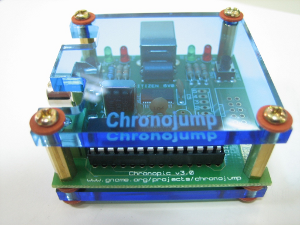
\includegraphics[width=250pt,height=188pt]{images/chronopic3}
\par\end{centering}

\caption{\label{fig:Chronopic3}Chronopic3.}
\end{figure}



\section{Chronopic connections}

Chronopic 3 is a USB powered hardware. Using USB cable it receives
data from PC and also power. To complete the connection, this cable
will also be connected to the socket.

There are two types of Chronopics:
\begin{itemize}
\item Multitest: Used in jumping and racing tests.
\item Encoder: Used to connect linear, rotary and friction encoders.
\end{itemize}
The first time you connect a Chronopic and open Chronojump a Chronopic
connection window will ask you to identify the type of Chronopic you
have connected.

\selectlanguage{spanish}%
\begin{figure}[H]
\begin{centering}
\includegraphics[width=0.5\columnwidth]{/home/xpadulles/chronojump-docs/images/chronopic-connection}
\par\end{centering}

\caption{\selectlanguage{british}%
\label{fig:chronopic-connection}Chronopic connection\selectlanguage{spanish}%
}
\end{figure}


\selectlanguage{british}%

\subsection{Multitest}

Chronopic will be connected to the contact platform or photocell barrier
through the RCA connection
\includegraphics[scale=0.03]{images/RCA_connector}
, the terminal block 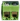
\includegraphics[scale=0.03]{images/screw_connector}
or both.

\selectlanguage{spanish}%
\begin{figure}[H]
\noindent \centering{}%
\begin{tabular}{|c|c|c|c|c|c|}
\hline 
\selectlanguage{british}%
Name\selectlanguage{spanish}%
 & \selectlanguage{british}%
USB-A\selectlanguage{spanish}%
 & \selectlanguage{british}%
USB-B\selectlanguage{spanish}%
 & \selectlanguage{british}%
RCA\selectlanguage{spanish}%
 & \selectlanguage{british}%
RCA 2-1 adaptor\selectlanguage{spanish}%
 & \selectlanguage{british}%
Plug\selectlanguage{spanish}%
\tabularnewline
\hline 
\hline 
\selectlanguage{british}%
Connected to:\selectlanguage{spanish}%
 & \selectlanguage{british}%
Computer\selectlanguage{spanish}%
 & \selectlanguage{british}%
Chronopic\selectlanguage{spanish}%
 & \selectlanguage{british}%
Device\selectlanguage{spanish}%
 & \selectlanguage{british}%
Device + RCA cables\selectlanguage{spanish}%
 & \selectlanguage{british}%
Electric socket\selectlanguage{spanish}%
\tabularnewline
\hline 
\selectlanguage{british}%
\selectlanguage{spanish}%
 & 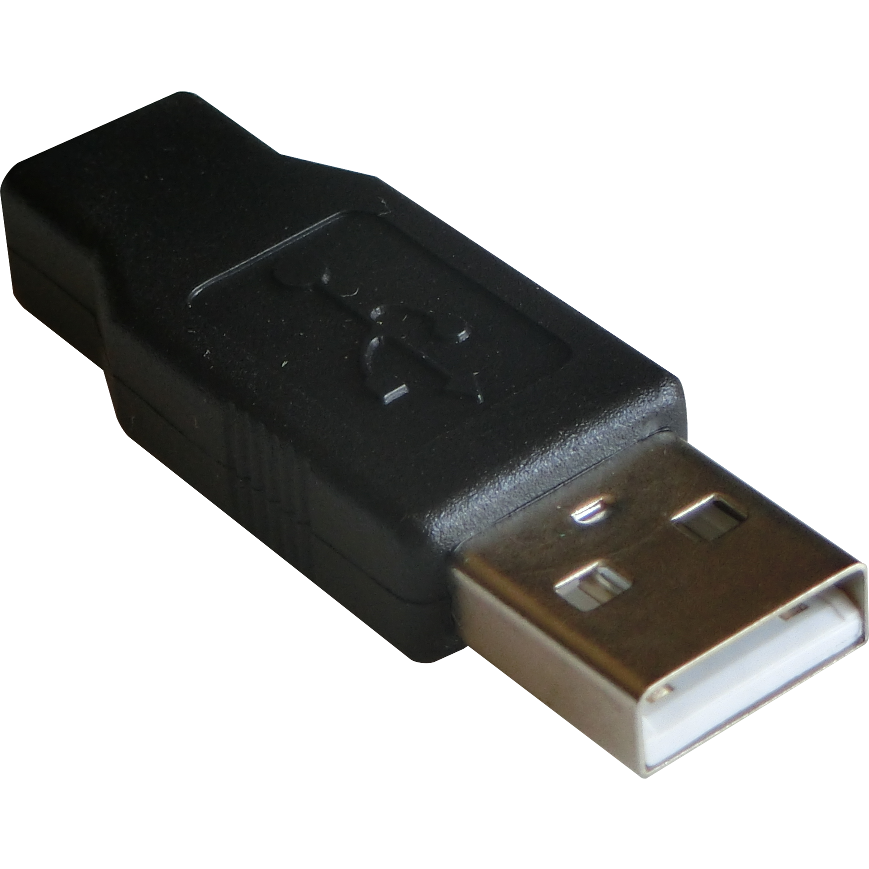
\includegraphics[scale=0.07]{/home/xpadulles/chronojump-docs/images/USB-A} & 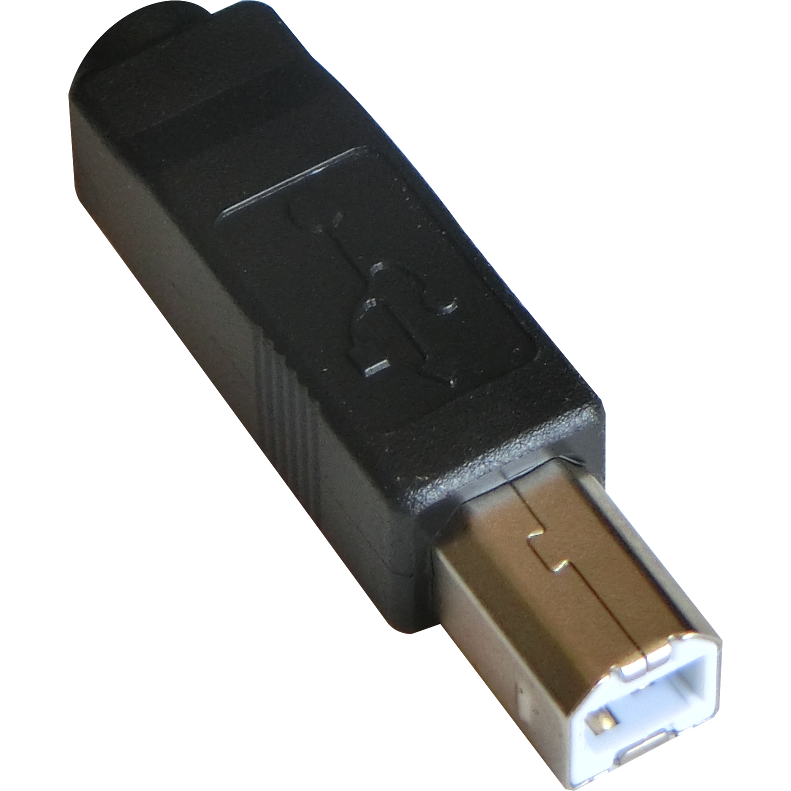
\includegraphics[scale=0.07]{/home/xpadulles/chronojump-docs/images/USB-B} & 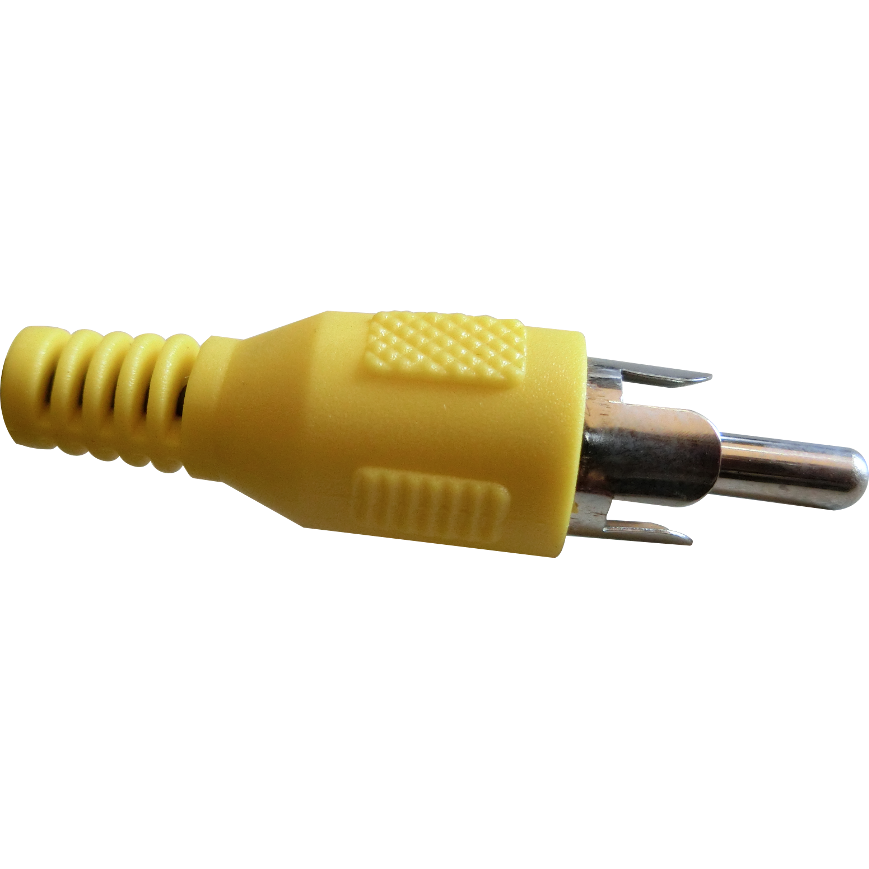
\includegraphics[scale=0.07]{/home/xpadulles/chronojump-docs/images/RCA} & 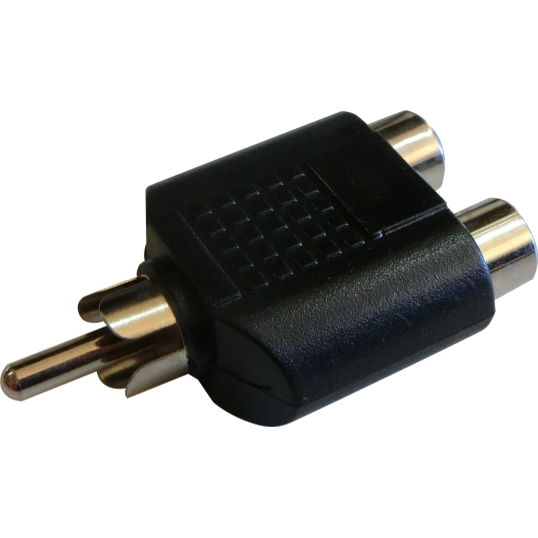
\includegraphics[scale=0.1]{/home/xpadulles/chronojump-docs/images/Adaptador-RCA.PNG} & 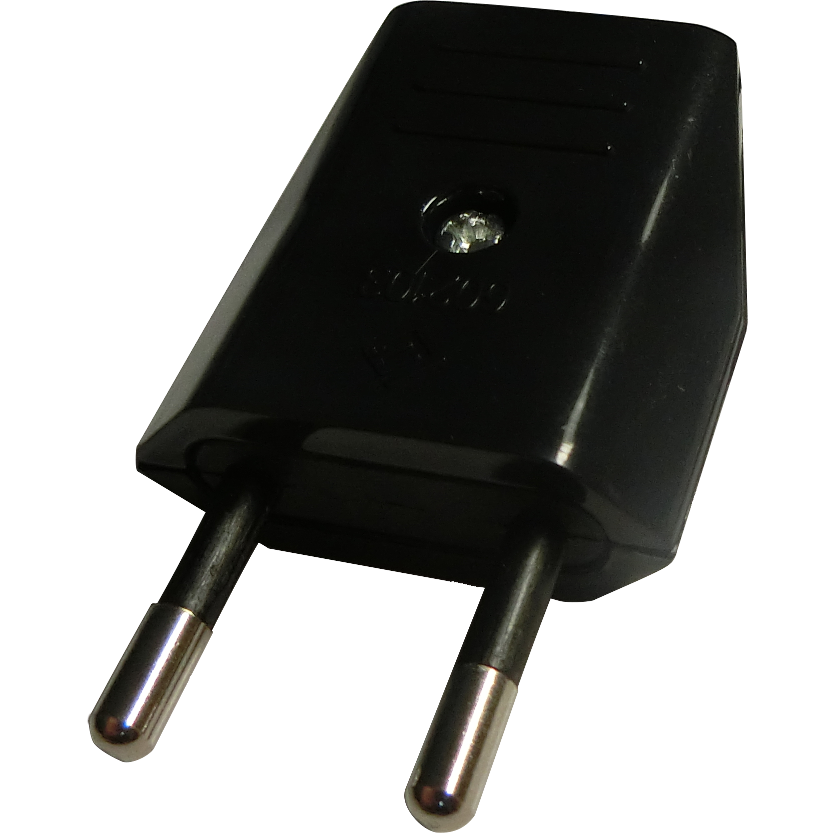
\includegraphics[scale=0.08]{/home/xpadulles/chronojump-docs/images/Photocel-Current}\tabularnewline
\hline 
\end{tabular}\caption{\selectlanguage{british}%
Multitest connections\selectlanguage{spanish}%
}
\end{figure}


\selectlanguage{british}%
Using Chronopic RCA (and / or fuse) it is possible to connect 'n'
networking platforms to any Chronopic. This model is useful to chronometer
situations where an athlete should not be able to be in more than
one platform at the same time. Both cables of each platform must be
connected to the RCA connector or the terminal block.

Software allows the connection up to 4 Chronopics with an independent
signal, each connected to one or more sensing devices. This makes
possible chronometer independently various subjects, complex paces
or other applications. 


\subsubsection{Chronopic working process}

Chronopic detect changes in the contact platform and sends it to the
computer by USB cable, USB-serial or serials. You can also use the
test button 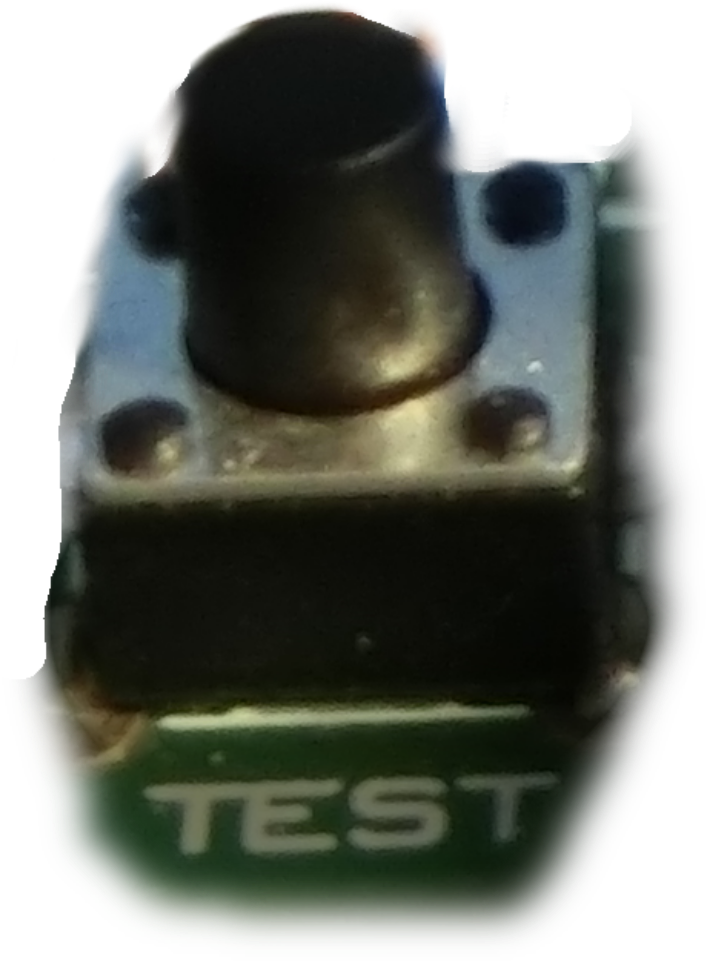
\includegraphics[scale=0.03]{images/test_button} to simulate
changes in the platform.

Chronopic has a green light to indicate when the subject is on the
platform or the photoelectric barrier (light stays off) or outside
(light is on).


\subsection{Encoder}

The encoder to Chronopic connection will be done with the RJ45 cable
of the encoder. The Chronopic to computer connection is made with
the USB A-B cable.

\selectlanguage{spanish}%
\begin{figure}[H]
\noindent \centering{}%
\begin{tabular}{|c|c|c|}
\hline 
\selectlanguage{british}%
USB-A (Computer)\selectlanguage{spanish}%
 & \selectlanguage{british}%
USB-B (Chronopic)\selectlanguage{spanish}%
 & \selectlanguage{british}%
RJ45 (Chronopic)\selectlanguage{spanish}%
\tabularnewline
\hline 
\hline 
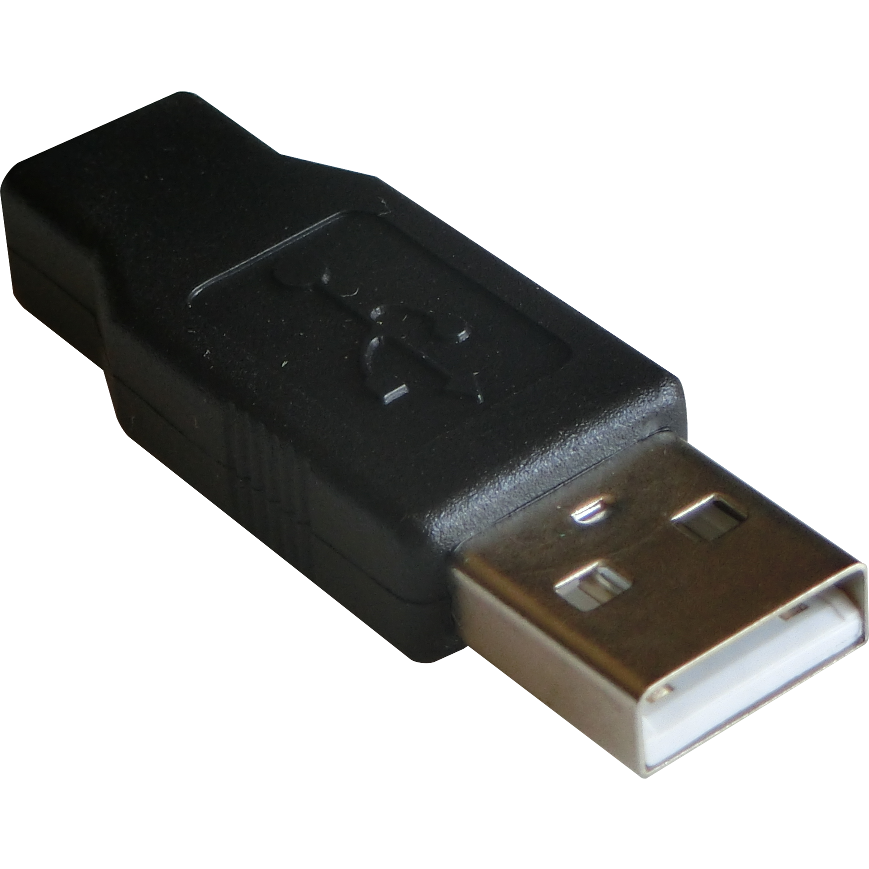
\includegraphics[scale=0.1]{/home/xpadulles/chronojump-docs/images/USB-A} & 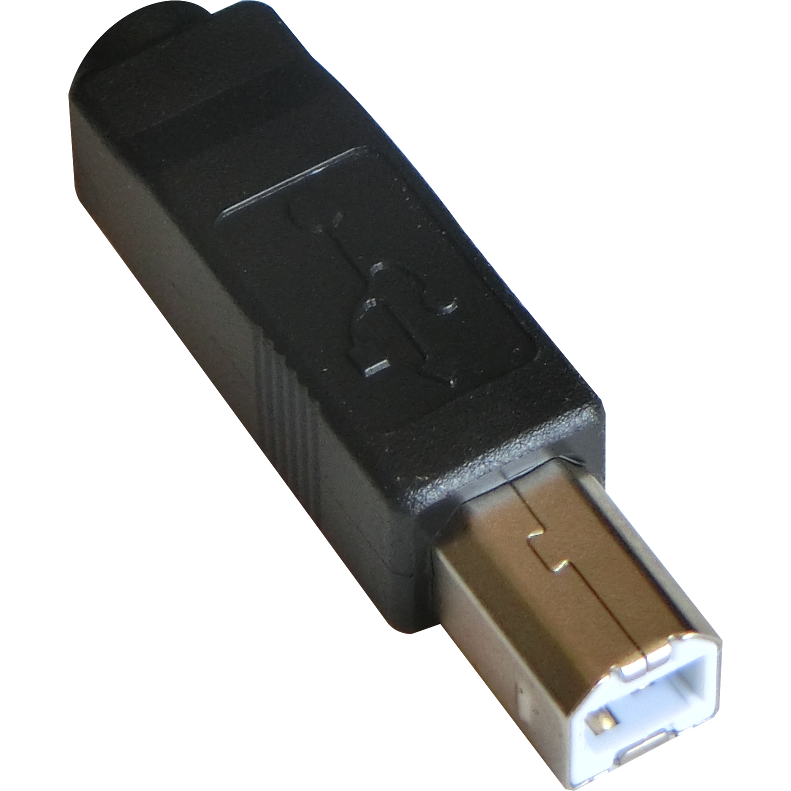
\includegraphics[scale=0.1]{/home/xpadulles/chronojump-docs/images/USB-B} & 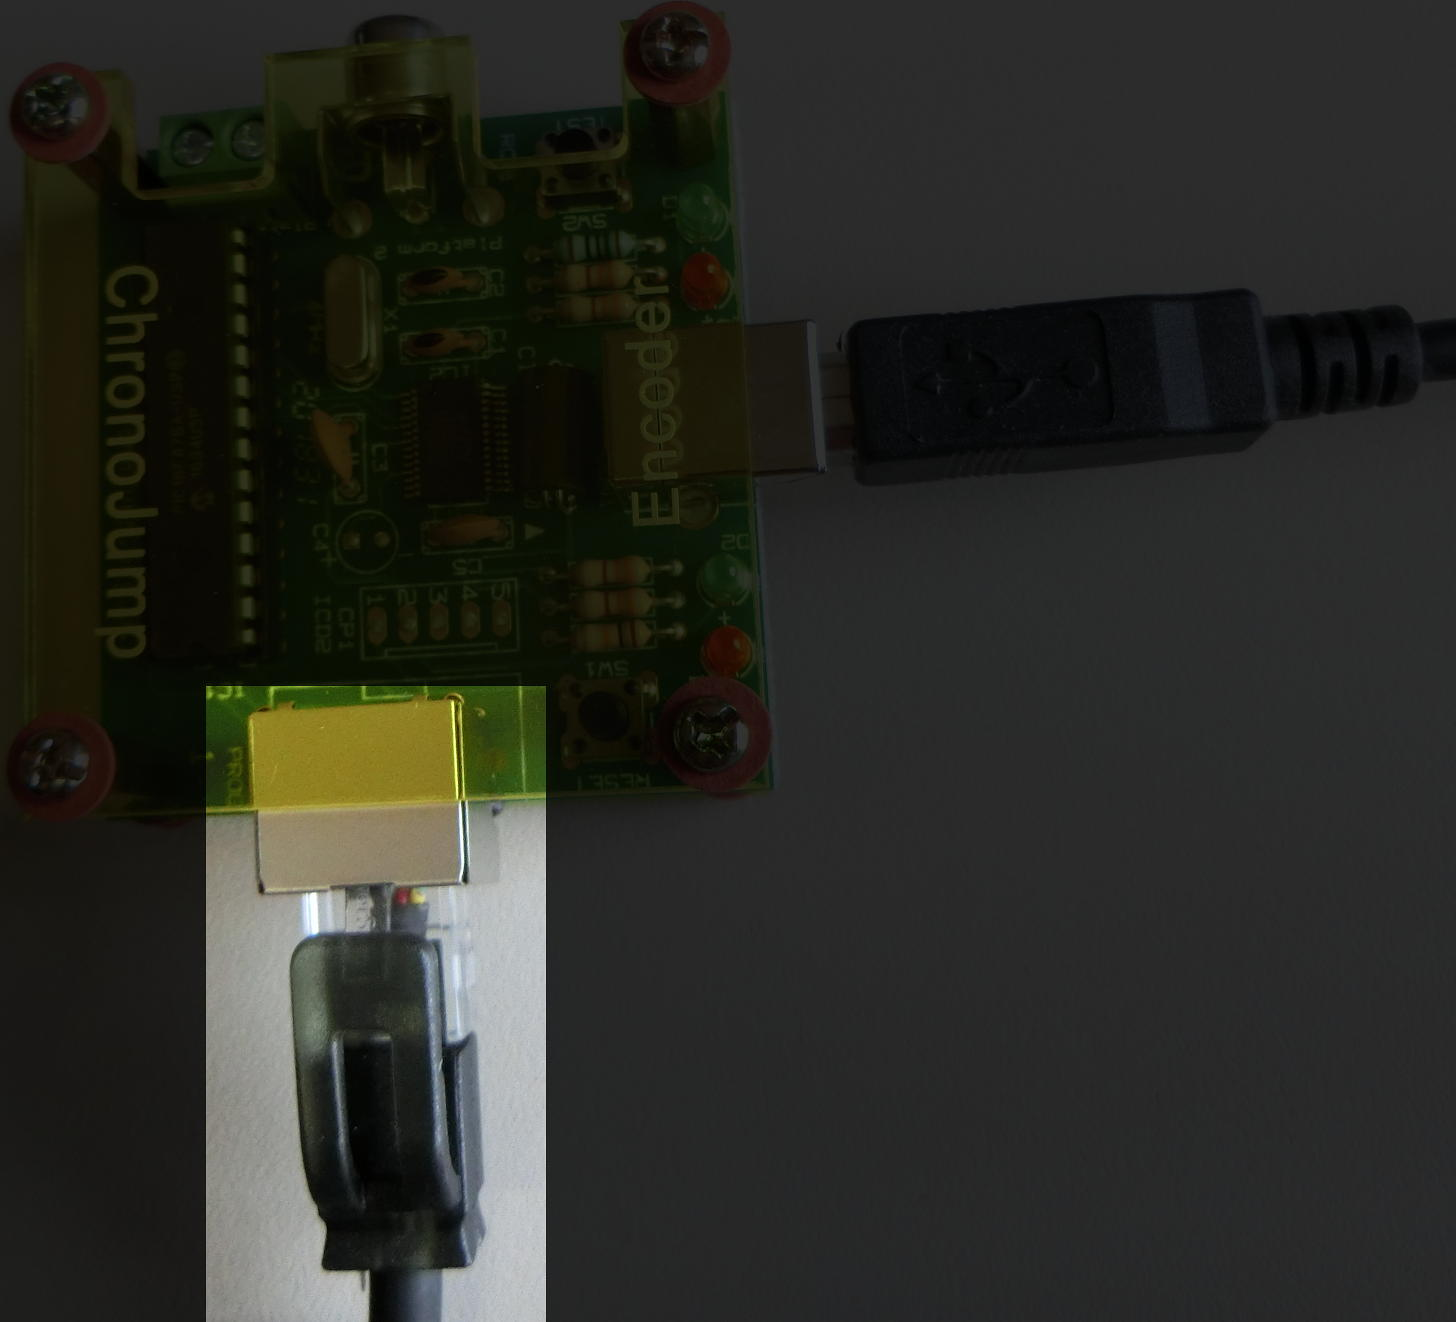
\includegraphics[scale=0.15]{/home/xpadulles/chronojump-docs/images/RJ45}\tabularnewline
\hline 
\end{tabular}\caption{\selectlanguage{british}%
Encoder Chronopic\selectlanguage{spanish}%
}
\end{figure}


\selectlanguage{british}%

\section{\label{sub:Chronopic-puertos-USB}USB ports}

The operating system assigns names to ports, as shown in Table \ref{tab:Nombres-de-puerto-USB}.

\begin{table}[H]
\begin{centering}
\begin{tabular}{|c|c|>{\centering}p{5cm}|>{\centering}p{4cm}|}
\hline 
Operating system & Port & Name & Comments\tabularnewline
\hline 
\hline 
MS Windows & USB & COM1, COM2, COM3, ... (seen to COM27) & Driver required\tabularnewline
\hline 
GNU/Linux & USB & \textbf{/dev/ttyUSB0}, /dev/ttyUSB1 & \tabularnewline
\hline 
Mac OSX & USB & /dev/tty.usbserial-{[}serial number{]} & Driver required\tabularnewline
\hline 
\end{tabular}
\par\end{centering}

\caption{\label{tab:Nombres-de-puerto-USB}Names of each operating system port.}


\noindent \centering{}The most common names are in bold type text.
\end{table}


The use of the driver is explained in the next section.


\subsection{Windows USB Driver}

A driver is a small program that indicates the computer how to operate
a new device. 

Chronopic plate requires a driver to run on Windows. This driver is
automatically installed when you install any version later than Chronojump
0.7.

If you connect the Chronopic to the computer, and it\textquoteright s
detected \textquotedbl{}New hardware found\textquotedbl{}, then the
driver is not required, in other case it will be necessary to run
the driver.


\section{\label{sub:Modificaci=0000F3n-del-puerto}Modification port assigned
by Windows}

If the port assigned is COM5 or higher it may cause problems in some
computers detection. If this happen, it\textquoteright s recommended
to assign a lower port than COM5, preferably COM1 or COM2.

To manually assign a port, repeat the steps described in \ref{sub:Detecci=0000F3n-del-puerto}
to know which port is assigned, then do the following steps:
\begin{enumerate}
\item Click \textquotedbl{}Port Settings\textquotedbl{}.
\item Click on \textquotedbl{}Advanced Options\textquotedbl{}.
\item Select one of the ports COM1-4 (preferably COM1 or COM2).
\item Accept and close the assistant.
\item Disconnect the USB cable and reconnect it after a few seconds.
\end{enumerate}
At this point it should be assigned a COM port that device that will
last forever. Alternatively, return to perform the steps described
in \ref{sub:Detecci=0000F3n-del-puerto} to verify that the change
was made directly. 

En este momento ya deber�a tener el puerto COM asignado para siempre
a dicho dispositivo. Opcionalmente, si quiere puede comprobar que
el cambio se ha realizado directamente puede volver a realizar los
pasos descritos en \ref{sub:Detecci=0000F3n-del-puerto}.


\section{Chronopic solution problems}

In case of detection failure when changing Chronojump platform, we
propose the following battery of tests. If Chronopic is not working
after performing these tests, please noted at the Forum \url{http://foro.chronojump.org}.

Perform each of the tests until it\textquoteright s working correctly.
Remember to check that the cables are connected properly. 
\begin{enumerate}
\item Power Problem: The red light will turn on when you connect the USB
cable (this will happen when the computer is turned on except when
there is a connected platform and someone stepping on it, or pushing
the test button 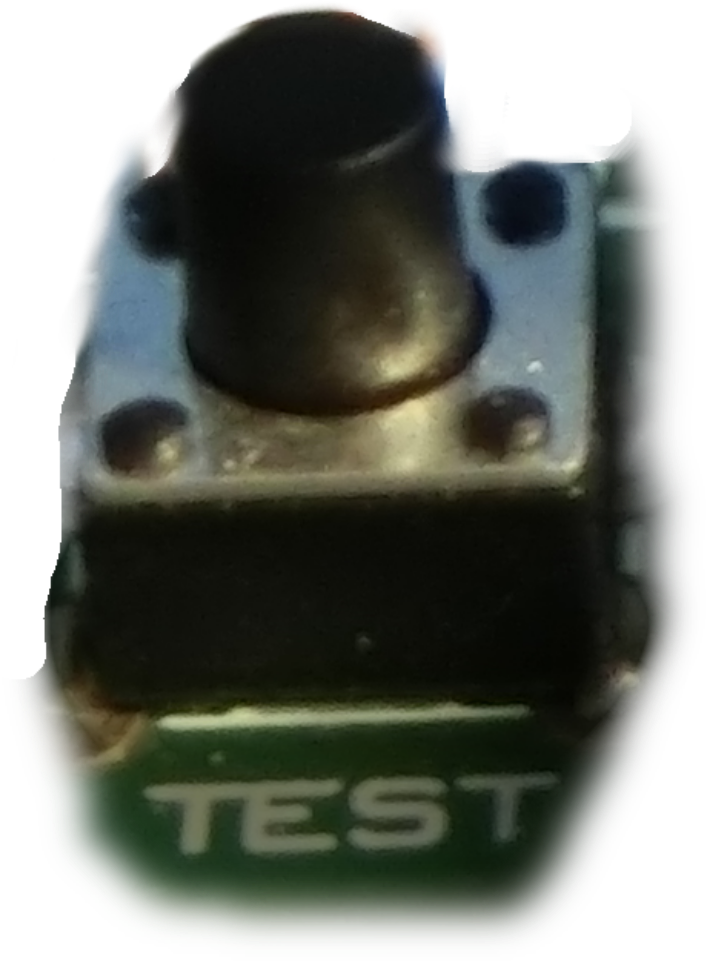
\includegraphics[scale=0.03]{images/test_button}).
\item Problem networking platform: Connect the contact platform to Chronopic
and the Chronopic to the computer (no need to open chronojump)and
check the Chronopic by clicking on the platform and checking if the
light turns on and off. If the light doesn\textquoteright t turn on
and off, but it did in the previous step, then the cables are in touch
when they are connected to Chronopic. Insulate them, check if they
are poorly connected or if the platform has a bad contact (disassemble
and repair).
\item Port problem on Windows: If the contact platform doesn\textquoteright t
have any problem, unplug it and continue the testing only with the
Chronopic. Then, check if the port is detected and connect the cables
to the computer, the power should also be detected in the Chronopic
as described in Section \ref{sub:Detecci=0000F3n-del-puerto}. Windows
may detect more than one type of port COM, do the following test to
both. If the port assigned is higher than COM4, it\textquoteright s
recommended to modify the port to one less than COM4, preferably COM1
or COM2 as described in Section \ref{sub:Modificaci=0000F3n-del-puerto}.
\item Execute Chronojump, select the port configuration in the Chronopic
window. A dialog will appear asking you to click \textquotedbl{}OK\textquotedbl{}
and after this click on the button Chronopic, shortly Chronopic should
be detected and ready to be used with the platform connected if desired.
\end{enumerate}

\part{Using Chronojump}


\chapter{Using Chronojump}

When Chronojump is opened, a window will allow you to select the type
of tests you are gone to work with.

\begin{figure}[H]
\begin{centering}

\includegraphics[width=1\columnwidth]{images/splash}
\par\end{centering}

\caption{\label{fig:splash}Chronojump splash screen.}
\end{figure}


Once you have selected, if you want to go back to this windows you
can go to \emph{Menu -> Mode: -> Main window}

You can also configure some parameters related to the automatic hardware
detection. If you experience problems at start or while capturing
try the different options.


\section{Chronojump main window}

When chronojump is opened you will be asked the mode you want to work
with. Chronojump has 4 modes and in each one there is a lot of diferent
tests. 

Figure \ref{fig:Ventana-principal-de} shows Chronojump main window.
This is divided into the following parts:
\begin{description}
\item [{The~menu}] where you find the access to session and help.
\item [{Edit~subject}] provides a quick access to individual operations.
\item [{Subject~selection}] where you can select the subject and edit
it with the menu that appears when you click on the right button of
the mouse.
\item [{Chart~selected~test}] If there is a drawing of the test selected
or targeted by the mouse, it will be shown. Also, if the program has
expanded information on the test, displays an icon to indicate it.
By pressing this button it will display a help window on this test
chart containing the expanded and test information.
\item [{Tabs}] that allow you to change the work form: Contacts (platform
of photocell), Encoder and Server.
\item [{Test}] type with the functionality of executing each of the tests
on the tab or active labor module.
\item [{Viewing~and~editing~the~tests}] shows different selectors for
viewing and editing the jumps and runs. User Notification displays
information about the last action.
\end{description}
\begin{figure}[H]
\begin{centering}
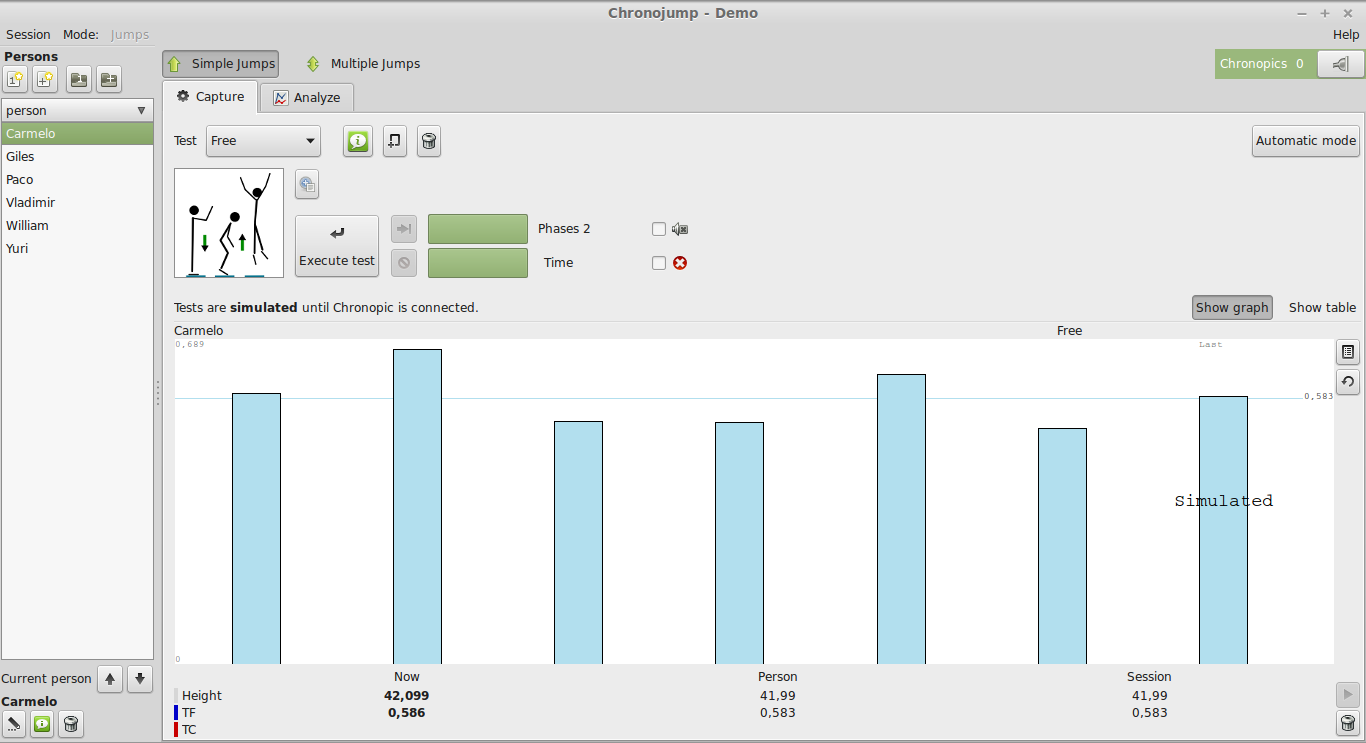
\includegraphics[width=1\columnwidth]{images/chronojump_main_window_english}
\par\end{centering}

\caption{\label{fig:Ventana-principal-de}Chronojump main window.}
\end{figure}



\section{Chronojump Menu}

In the following pictures you can see the drop down menu of the program.
\begin{description}
\item [{Session~Menu}] see figure \ref{fig:menu_session}.
\item [{Mode~Menu}] see figure \ref{fig:menu_mode}.
\item [{Help~Menu}] (Top-right corner of the window) see figure \ref{fig:menu_help}.
\end{description}
\begin{figure}[H]
\begin{centering}
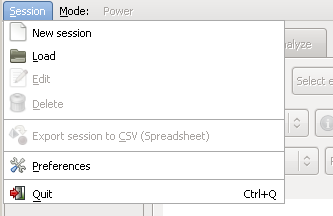
\includegraphics[scale=0.6]{images/menu_session}
\par\end{centering}

\caption{\label{fig:menu_session}Session Menu.}
\end{figure}
\begin{figure}[H]
\begin{centering}
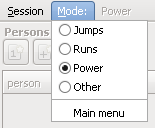
\includegraphics{images/menu_mode}
\par\end{centering}

\caption{\label{fig:menu_mode}Mode Menu.}
\end{figure}
\begin{figure}[H]
\begin{centering}

\includegraphics[scale=0.6]{images/menu_help}
\par\end{centering}

\caption{\label{fig:menu_help}Help Menu.}
\end{figure}



\section{Chronopic/s Connection.\label{sec:Chronopic/s_connection}}

Is possible to connect one or more Chronopics on the menu: \emph{Tools
/ Chronopic}. In Figure \ref{fig:Chronopic-connection} two Chronopics
connected are shown. The connection to the Chronopic timer is specifically
addressed in section \ref{par:Chronopic:-concepto-y-configuracion}.

The first time a Chronopic is connected to a computer, the typ of
Chronopic (Jumps/Races or Encoder) must be configured. This configuration
will be stored for future Chronojump use. Chronojump will detect automatically
all the Chronojump previously configured.

\begin{figure}[p]
\begin{centering}
\includegraphics[scale=0.6]{images/chronopic-connection}
\par\end{centering}

\caption{\label{fig:Chronopic-connection}Chronopic connection.}


\noindent \centering{}The figure corresponds to the program Chronojump
whith two connected Chronopics.
\end{figure}



\section{Database: sessions, subjects and tests}

Chronojump stores all data in one database file. Thus, instead of
collecting the information in individual files for each session, all
information is organized in a single file to facilitate the study
of relationships between:
\begin{itemize}
\item sessions
\item people
\item tests (jumping, running, reaction times, pulses (rates), multi Chronopic)
\end{itemize}
All modifications in session, subjects and tests, will be updated
at any time in the database. So there isn\textquoteright t need to
save the information periodically and make data loss to a computer
error. If rare case, the program crash, you wouldn\textquoteright t
lose any data except sometimes the one that is being performed at
the time.


\subsection{Sessions}

The sessions represent situations where the coach or evaluator gathers
many athletes (subjects) for a series of tests. Every time you gather
a group of athletes to be tested in a short space of time (usually
one day), you should create a new session. Although the subjects to
assess are the same as in other session, you should create a new one
to keep adding subjects and tests in an old session. In this way,
you can make comparisons between data.

Figures \ref{fig:Nueva-sesi=0000F3n.-Alumnos} and \ref{fig:Nueva-sesi=0000F3n.-Deportistas}
demonstrate the creation of a session.

\begin{figure}[H]
\noindent \begin{centering}
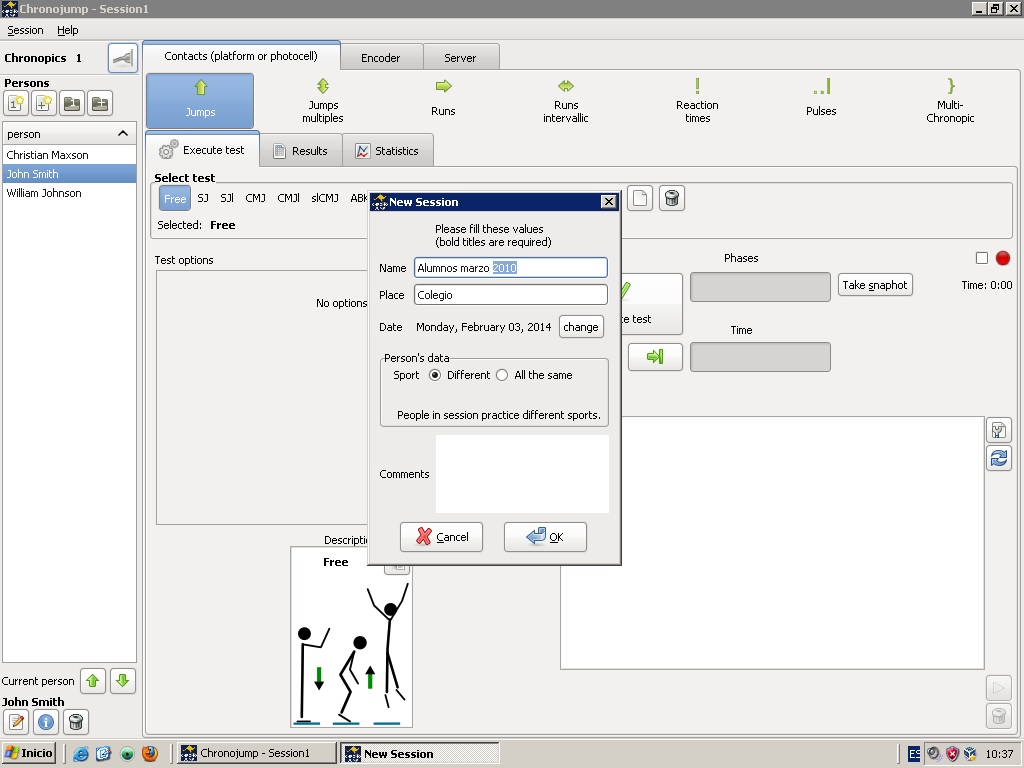
\includegraphics[scale=0.6]{images/nueva_sesion_colegio}
\par\end{centering}

\caption{\label{fig:Nueva-sesi=0000F3n.-Alumnos}New Session. School students.}
\end{figure}


\begin{figure}[H]
\noindent \begin{centering}
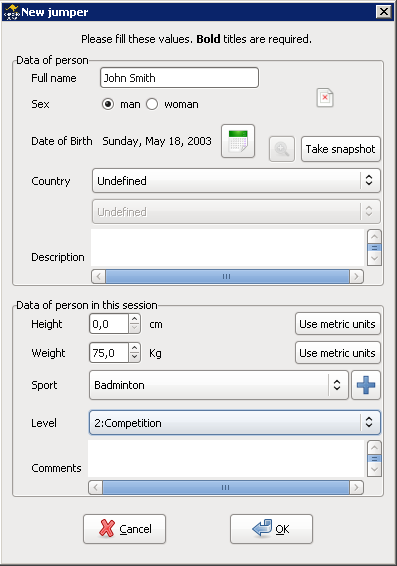
\includegraphics[scale=0.6]{images/nueva_sesion_artistica_competicion}
\par\end{centering}

\caption{\label{fig:Nueva-sesi=0000F3n.-Deportistas}New Session. Rhythmic
competitors.}
\end{figure}



\subsubsection{Creation}

Click on the menu \emph{Session menu / Create session} and one window
will be opened where you must enter the name of the session, the date
and the sport practiced. Optionally you can also indicate the place
where is done and even add comments.


\subsubsection{Load}

If you want to load a session already created to study, add subjects
and / or to test, click on the \emph{Session menu / Load session}.
It will show a list of sessions created and information of the subjects
enrolled in each of them and the tests performed.


\subsubsection{Edici�n}

Click on \emph{Session menu / Edit session} to modify the parameters
that have been inserted earlier. Normally, it\textquoteright s used
the edition of sessions to add comments about the evolution.


\subsubsection{Delete}

To delete a \textbf{session and all tests} performed, click on the
\emph{Session menu / Remove session}. A confirmation window will appear. 


\subsection{subjects}

All individuals able to perform the tests are known as subject. It\textquoteright s
strongly recommended to create one subject only once in order to study
the evolution over time. In following sessions the subject must be
loaded.

Figure \ref{fig:Creaci=0000F3n-de-un-sujeto} shows the creation of
a person.

\begin{figure}[H]
\noindent \begin{centering}
\includegraphics[scale=0.6]{\string"images/Captura-Nuevo saltador\string".png}
\par\end{centering}

\caption{\label{fig:Creaci=0000F3n-de-un-sujeto}Creation of a person.}
\end{figure}



\subsubsection{Current person}

The subject on the left side of the main window is known as \emph{current
person}. All tests done shall be linked to that subject. The latter
subject created or loaded is assigned as current person. 

Tests shall not start until the current person is assigned.


\subsubsection{Creation}

Click on the \emph{Person menu / Create person} or use the Create
button to create a person. You may indicate the full name, gender,
date of birth, height, weight, country, sport, mode and level. It\textquoteright s
important to enter the full name to avoid further conflicts with other
different subjects.

In order to accelerate the creation of multiple subjects, click on
the menu \emph{Subject / Create subjects {[}multiple{]}}. A window
will appear where you can create multiple subjects at once. You can
choose between \emph{Add entries from CSV (spreadsheet)} or \emph{Add
entries manually}.

In the first case you will need a coma separated value file (.csv)
previously created with the information of the name, surname, genre
and weight in diferent fields. The format of the file can be specified
with headers 
\includegraphics[scale=0.75]{images/import_headers}
or without it 
\includegraphics[scale=0.75]{images/import_no_headers}.
Additionally you can have a file with a single column for the full
name 
\includegraphics[scale=0.75]{images/import_1_field} or two columns
for the name and surname 
\includegraphics[scale=0.75]{images/import_2_fields}.

In the second case, you can create manually a set of subjects as shown
in the figure.

Once created, if you still want to create more subjects, you can click
again on the same menu item. Figure \ref{fig:Creation of multiple subjects}
shows the creation of 11 subjects at once.

\begin{figure}[H]
\noindent \begin{centering}
\includegraphics[scale=0.5]{\string"images/Captura-Cargar atletas\string".png}
\par\end{centering}

\caption{\label{fig:Creation of multiple subjects}Load subjects.}
\end{figure}



\subsubsection{Load}

If a person has participated in another session, and you want to evaluate
him/her again in the current session, click on \emph{Load person},
and enter the same subject to the new session. The program will distinguish
between tests (jump, run, reaction times and rhythms) made by the
same person in two or more sessions.

If you created a session and you want to continue with the same person/s
in another session click \emph{Load subjects from another session}
and check all subjects who participated in the other session or multiple
session. If you wish you can always discard any subject.

Figures \ref{fig:Cargar-atletas} and \ref{fig:Cargar-atletas-otra_sesion}
show the load of subjects.

\begin{figure}[H]
\noindent \begin{centering}
\includegraphics[scale=0.5]{\string"images/Captura-Cargar atletas\string".png}
\par\end{centering}

\caption{\label{fig:Cargar-atletas}Load subjects.}
\end{figure}


\begin{figure}[H]
\noindent \begin{centering}
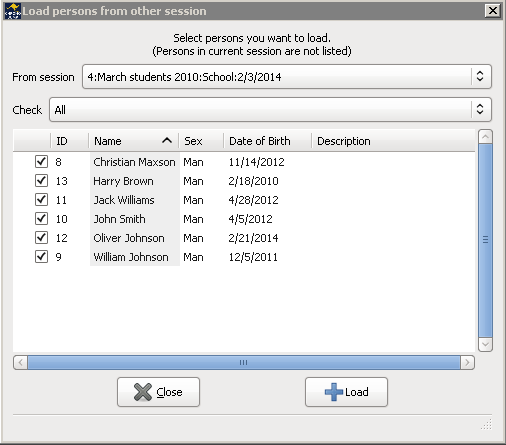
\includegraphics[scale=0.5]{images/Captura-Cargar_atletas_otra_sesion}
\par\end{centering}

\caption{\label{fig:Cargar-atletas-otra_sesion}Load subjects from other session.}
\end{figure}



\subsubsection{View subject tests}

Click \emph{Show all tests of current person }to see all the tests
that this person has done in the different sessions. You can also
select other subjects of the current session.


\subsubsection{Edit}

Click \emph{Edit person} or press \emph{p} (person) to modify the
data that was entered at the same time as the creation. You can also
add comments.


\subsubsection{Delete}

Click \emph{Delete current person} to be removed of the session. This
operation will remove all tests from any person in the current session.
It\textquoteright s important to know that the subject will not be
removed from the database and the tests in other sessions remain intact.

After deleting this subject, another subject will become the \emph{current
person}. Otherwise any test can be provided.


\subsection{Tests}

So far Chronojump manages five types of tests: jumping, running, reaction
times, rhythms and MultiChronopic. Later Chronojump can handle other
tests. These tests are detected by the signals sent by the contact
platform when the subject steps on and off it.

The database stores the tests and links to other data tables.


\chapter{Tests}

At the following text, it describes the management of the all types
of tests allowed in Chronojump software.


\section{Jump tests}

There is basically two types of jumps: simple and repetitive. Chronojump
detect a \textbf{single jump} as one phase of flight. That\textquoteright s
why there are two types of simple jumps:
\begin{enumerate}
\item Those who start and finish on the platform (single hop).We obtain
the variable flight time (TF) 
\item Those who started outside the platform (drop from a height or do a
jump before) to fall on the platform and then jump. Variables obtained:
Contact time (TC) (time between reception and takeoff on the platform)
and flight time (TF). Usually jumps will pursue minimum contact time
and maximum flight time as a power indicator.
\end{enumerate}
A \textbf{multiple jump} (also called reactive) is when you obtain
more than one flight time. For example: make two consecutive jumps
initiated on the platform in the order TF, TC, TF or start outside
the platform and continue with the order TC, TF, TC, TF.

Assuming that the body during the takeoff position is the same as
in the landing, the flight time indicatives the height of center of
gravity of the athlete in this jump.

Videotutorial: Right execution of the Bosco Tests \url{https://youtu.be/wa6-KgTOwkw}


\subsection{Simple jumps execution}

From the Simple Jumps button, you can select from the drop-down list
the following options:
\begin{itemize}
\item Free, normal jump without restriccions
\item \emph{SJ}, Squat Jump
\item \emph{SJ}l, Squat Jump with extra load (extra weight)
\item \emph{CMJ}, countermovement jump
\item CMJl, coutermovement jump with extra load (extra weight)
\item \emph{ABK}, jump with arms Abalakov
\item \emph{ABKl}, jump with arms Abalakov with extra load (extra weight)
\item \emph{D}Ja, drop jump with arms using
\item DJna, drop jump without arms using
\item \emph{Rocket,} Rocket Jump is simple jump similar to the squat jump
but it starts with a full flexion of the legs.
\item \emph{TakeOff}, only records the contact time
\item \emph{TakeOffWeight}, take off with extra load. It only records the
contact time
\item \emph{slCMJleft}, left leg countermovement jump.
\item \emph{slCMJright}, right leg countermovement jump.
\end{itemize}
Sometimes you will be asked to provide additional information as the
extra weight of the subject (SJL) or the height of the drop (DJ). 

The original protocol of Bosco for the \emph{DJ} test indicates that
the arms don\textquoteright t participate in the jump. Instead many
coaches ask their athletes to use the arms because is more similar
to the techniques used in sports. The original \emph{DJ} is called
\emph{DJna} (no arms), while the \emph{DJ} with arms is called \emph{DJ}a.
When you start a DJ test, the program will ask whether to use arms
or not and automatically appoint the jump properly.

If Chronopic has not been connected and activated from Chronopic window,
a jump will be simulated. In the other hand, if Chronopic is connected,
real jump will be done. Note that for some jumps the athlete should
be on the platform, while other jumps it\textquoteright s essential
to be elsewhere. You will be notified if the athlete's situation is
not correct. The progress barr shows the progress of the jump, which
may be stopped by clicking on the \emph{Finish} or \emph{Cancel} button.


\subsubsection{Automatic mode}

In order to accelerate the process of testing multiple subjects you
can click on the \emph{Automatic mode} button. This mode allows you
to perform tests creating or loading sequences of diferent jumps or
people.

Defining the sequence can be done either loading a preconfigured one
(\emph{Load sequence}) or creating a new one (\emph{Create new sequence).}

When a new sequence is created the order of the test must be defined.
There are three different options:
\begin{itemize}
\item \emph{By persons}: Each person of the session performs all the tests
before changing to the next person. Example: \emph{Chronojump profile}.
\item \emph{By tests}: Each test in the sequence is perfomed by all the
people in the session before changing to the next test. Example: \emph{Bilateral
profile by persons}
\item \emph{By sets}: Each person of the session performs the first set
of tests before changing to the second set of tests. It can be defined
up to 3 different sets of tests. Example: \emph{Bilateral profile
by sets}
\end{itemize}
To define a new sequence click on the type of sequence it is about
to be created and click on the \emph{Next }button. Then, in the new
window, the order of the tests can be defined. If the \emph{By sets}
option was selected, each set must be defined separately.

After defining the sequence, it can be saved clicking on the \emph{Save}
button.

Once the \emph{Next} button is pressed a new windows will show the
whole sequence indicating the order of the person and the test.

When the \emph{Accept} button is pressed the automatic mode is activated.
In this mode the person frame will be disabled and the name of the
next jumper and what test is going to be done will be shown in the
upper left corner of the Capure frame. The selection of the test will
also disappear, not allowing to change

After performing each jump test, the person and the test will change
automatically.

Clicking on the \emph{See order} button
\includegraphics{images/automatic_list}
the whole sequence of the test can be viewed.

To skip all the tests of a person and execute it at the end of the
sequence click on the \emph{Skip} 
\includegraphics{images/automatic_skip}.

To delete a person from the sequence click on \emph{Remove} button

\includegraphics{images/automatic_delete}.

Clicking on the \emph{End automatic mode} will return to the normal
way of work of Chronojump, allowing you to select the person and the
test to be performed.


\subsection{Repetitive jumps execution}

Click in the button on the Repetitive jumping tab:
\begin{itemize}
\item \emph{RJ(j)}, Repetitive Jump (jumps) or repetitive jumping limited
number of hops
\item \emph{Rj(t)}, Repetitive Jump (time) or time-limited repetitive jumping
\item \emph{RJ(unlimited}), unlimited repetitive jumping.
\item \emph{RJ(hexagon)}, reactive jump on an hexagon until three full revolutions
are done.
\item \emph{Triple jump}, triple jump starting from a falling height
\item \emph{Unlimited multiple jump with extra load}
\end{itemize}
Sometimes is necessary to provide additional information as the height
of the initial drop, the extra weight or value of the limiting factor
(hops or seconds). Click on \emph{More} to get a list of all the available
of the reactive jumps and execute them clicking OK. The jump menu
also provides access to these actions.

If Chronopic has not been connected and activated from Chronopic window,
a jump will be simulated. In the other hand, if Chronopic is connected,
real jump will be done. Note that for some jumps the athlete should
be on the platform, while other jumps it\textquoteright s essential
to be elsewhere.

If you want to execute the same type of jump to various subjects and
you don\textquoteright t want a button (only available on the tab
more), you can change the subject and use the Last button to allow
another person to perform the same jump.


\subsection{Auditive and visual feedback in repetitive jumps: bells }

In order to add a visual and auditory feedback during execution of
the jumps, you can set values of flight time, contact time, or the
relationship of both. To be shown a red bell (poor performance) or
green (good performance) together with a distinctive sound. Click
on the \textquotedbl{}Bells\textquotedbl{} to configure these actions
as shown in Figure \ref{fig:Campanas---feedback}.

\begin{figure}[H]
\noindent \begin{centering}
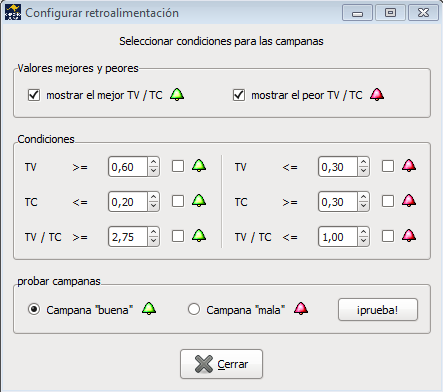
\includegraphics[scale=0.6]{images/campanas_es}
\par\end{centering}

\caption{\label{fig:Campanas---feedback}Bells - auditive and visual feedback.}
\end{figure}



\subsection{\noindent Chronojump profile}

Chronojump incorporates a quick method for generating an athlete profile
in which different variables are shown:
\begin{itemize}
\item Maximum force: Hability of moving an load equal to the double of the
body weight.
\item Explosive force: Hability of moving a load equal to the body weight.
\item Elasticity: Force increment due to the elastic energy acumulated during
the shortening-stretching cycle.
\item Arms using: Force increment due to the arms using.
\item Reacitve reflex: Force increment due a previous falling from certain
heigth (activation of reflex mechanisms)
\end{itemize}
In order to generate a complete profile it is necessary to have been
performed this jumps:
\begin{itemize}
\item SJl with an external load equal to the body weight.
\item \noindent SJ
\item \noindent CMJ
\item \noindent Abalakov
\item DJ with a falling height near the one that generates the maximum jump
height.
\end{itemize}
\noindent Si desea ver el perfil de un atleta haga clic en la pesta�a
de \emph{Perfil de saltos.}

To generate the Jumps profile go to Jumps profile tab.

\begin{figure}[H]
\noindent \begin{centering}
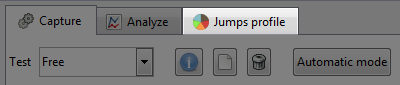
\includegraphics{/home/xpadulles/chronojump-docs/images/chronojump_profile_tab}
\par\end{centering}

\caption{\selectlanguage{spanish}%
Jumps profile tab\selectlanguage{british}%
}
\end{figure}


Once there, and if al the jumps are performed a graph similar to this
will be shown.

\begin{figure}[H]
\noindent \begin{centering}
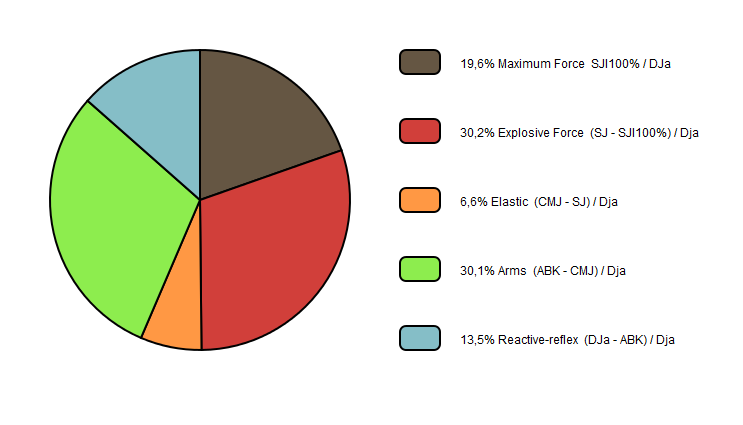
\includegraphics[scale=0.5]{/home/xpadulles/chronojump-docs/images/chronojump_profile}
\par\end{centering}

\caption{\selectlanguage{spanish}%
Chronojump jumps profile\selectlanguage{british}%
}
\end{figure}



\subsection{Jumps view}

Simple jumps are shown on the \emph{Jumps} tab and the reactive Jumps
on the \emph{Jump Reactive} tab. In both cases, it\textquoteright s
included a filter for all the possible tests or only a particular
type.

Tests are associated with the jumpers. The order of the tests presentation
of each jumper is chronological so, the last test appears at the end
of the list. It\textquoteright s included a button that allows sorting
the tests by the type of jump and not in chronological order.

All jumps are selected in the view filter. A series of values are
presented at each hop. It\textquoteright s possible to change the
view by accessing at the Preferences (more information in section
\vref{sec:Preferencias}).

You can use the \emph{magnifying glass} button (or press \emph{z})
to facilitate the view of the tests.


\subsection{Jumps edition}

You can add comments to a jump or change the person (if you forgot
to change the current person previously) If you select the desired
jump and click on the Edit button on the selected jump, you can also
find it on the menu, or by pressing the button \emph{e}.

In the reactive jumps, since they are composed of a set of jumps,
this change will affect all the jumps even if only one is selected.


\subsection{Repair repetitive jumps}

Using \emph{Repair selected} button or pressing \emph{r}, you can
add a jump, modify a contact time or flight time or delete a jump.
If a repetitive jump type has been defined to be limited to max \emph{n}
jumps, or max \emph{n} seconds, this conditions will limit the repair
functionality. When this happens, you will find an information text
on the bottom of the window.


\subsection{Jumps delete}

To delete a jump, select it and click the \emph{Delete selected jump}
button. Its equivalent in the menu or press \emph{d} (delete). By
deleting the test you will be asked to confirm it if the delete confirmation
option is activated in the \emph{Preferences} menu (more information
in section \vref{sec:Preferencias}).

Deleting a repetitive jump will delete all it's jumps.


\subsection{Creation of new jump types}

In order to adapt the software to the needs of each user, it has been
included the function: \emph{Add jump type} (on \emph{Jumps} menu).
This allows trainer to define easily and powerully the desired jump
types.

Created jump type will be available on database to be used at any
session, and it will be listed clicking on the \emph{More} button
at the \emph{Jump} or\emph{ Jump repetitive} tabs (depending on which
kind of jump it's created). This new jump type will be also differentiated
on statistics, graphs and reports.

On creation, you should give it a distintive name and classify between
simple or repetitive. If jump is repetitive, then you can limit is
by jumps, time, or leave it unlimited.

The limit by time or jumps options can be defined as a fixed value
or leaved as undefined. If it's defined fixed, all new jumps of this
type will be limited to that value; in the other hand, if the type
is not fixed, user will be asked by limit value everytime a new jump
is done.

Last settings include: start inside or outside the platform, allow
to jump with an extra weight, and add a description to the jump type.
In the figure \ref{fig:Creaci=0000F3n-de-nuevo-tipo-salto} you can
see the creation of new jump type.

\begin{figure}[H]
\begin{centering}
\includegraphics[scale=0.6]{\string"images/Captura-Crear un tipo de salto nuevo\string".png}
\par\end{centering}

\caption{\label{fig:Creaci=0000F3n-de-nuevo-tipo-salto}Creation of a new jump
type.}
\end{figure}



\subsection{Examples on creation of new jump types}

Here you can find some examples on creating new jump types. The names
of the types have been invented in this manual. The table \ref{tab:Created-jump-type-examples}
is also useful to understand the different variables.
\begin{itemize}
\item \emph{``SJ-N''} Jump like Squat Jump but the hands are on the nape
instead of hips.
\item \emph{``DJ-Rope2''} Jump like Drop Jump but after executing the
Drop jump, person have to jump again doing two turns with the skipping
rope on the air.
\item \emph{``Triple''} Repetitive jump starting outside the platform
and including three jumps.
\item \emph{``50\%fatigue''} Repetitive jump that has to be done until
arriving to 50\% of the person's fatigue. The number of seconds needed
to be fatigued is personal and is known previously by the trainer.
Starts inside.
\item \emph{``RopeUnlimited''} Person has to jump the rope until trainer
(or jumper) decides to finish. Start inside the platfom and can be
done with an extra weight.
\end{itemize}
\begin{table}[H]
\begin{centering}
\begin{tabular}{|c|c|c|c|c|c|}
\hline 
Name & Tipe & Limited by & Fixed & Start in & Additional weight\tabularnewline
\hline 
\hline 
SJ-N & Simple & - & - & Yes & No\tabularnewline
\hline 
DJ-Rope2 & Simple & - & - & No & No\tabularnewline
\hline 
Triple & Repetitive & Jumps & Yes(3) & No & No\tabularnewline
\hline 
50\%fatigue & Repetitive & Time & No & Yes & No\tabularnewline
\hline 
RopeUnlimited & Repetitive & Unlimited & - & Yes & Yes\tabularnewline
\hline 
\end{tabular}
\par\end{centering}

\caption{\label{tab:Created-jump-type-examples}Examples on jump types created
by user.}
\end{table}



\section{Races}

\begin{figure}[H]
\begin{centering}
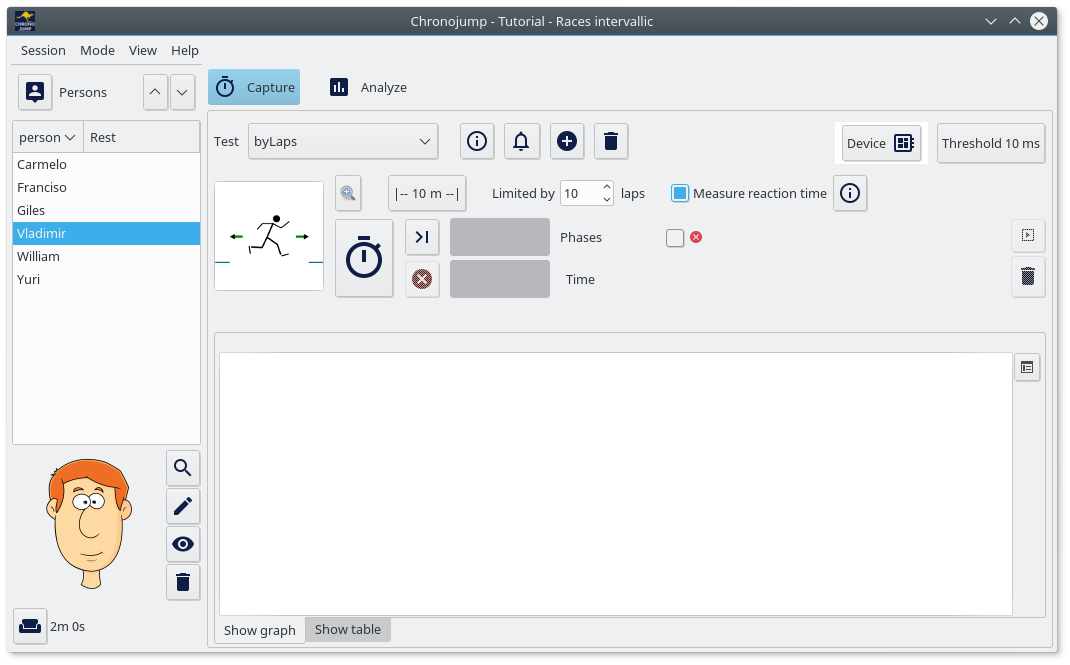
\includegraphics[width=0.6\columnwidth]{images/races}
\par\end{centering}

\caption{\label{fig:Schem-two-photo-1}Drawing of two barriers and a switch
to measure races.}
\end{figure}


Running can be detected by three kind of devices:
\begin{itemize}
\item platform/s
\item photocell/s
\item push button/s
\end{itemize}
On a run test Chronojump detects time between detection devices. If
the run is ``circular'', it can be used a single device (platform,
photocell or push button), in the other circuits, there's a need of
more than one detection device (of any type).

From now on, \emph{device in contact} means that the person is on
the platform or blocking a photocell signal or pressing the push button.
Is important to note that the person should never be in contact in
more than one device at the same time.

The figure \ref{fig:Schem-two-photo} shows a drawing of the position
of two platforms to measure run.

\begin{figure}[H]
\begin{centering}
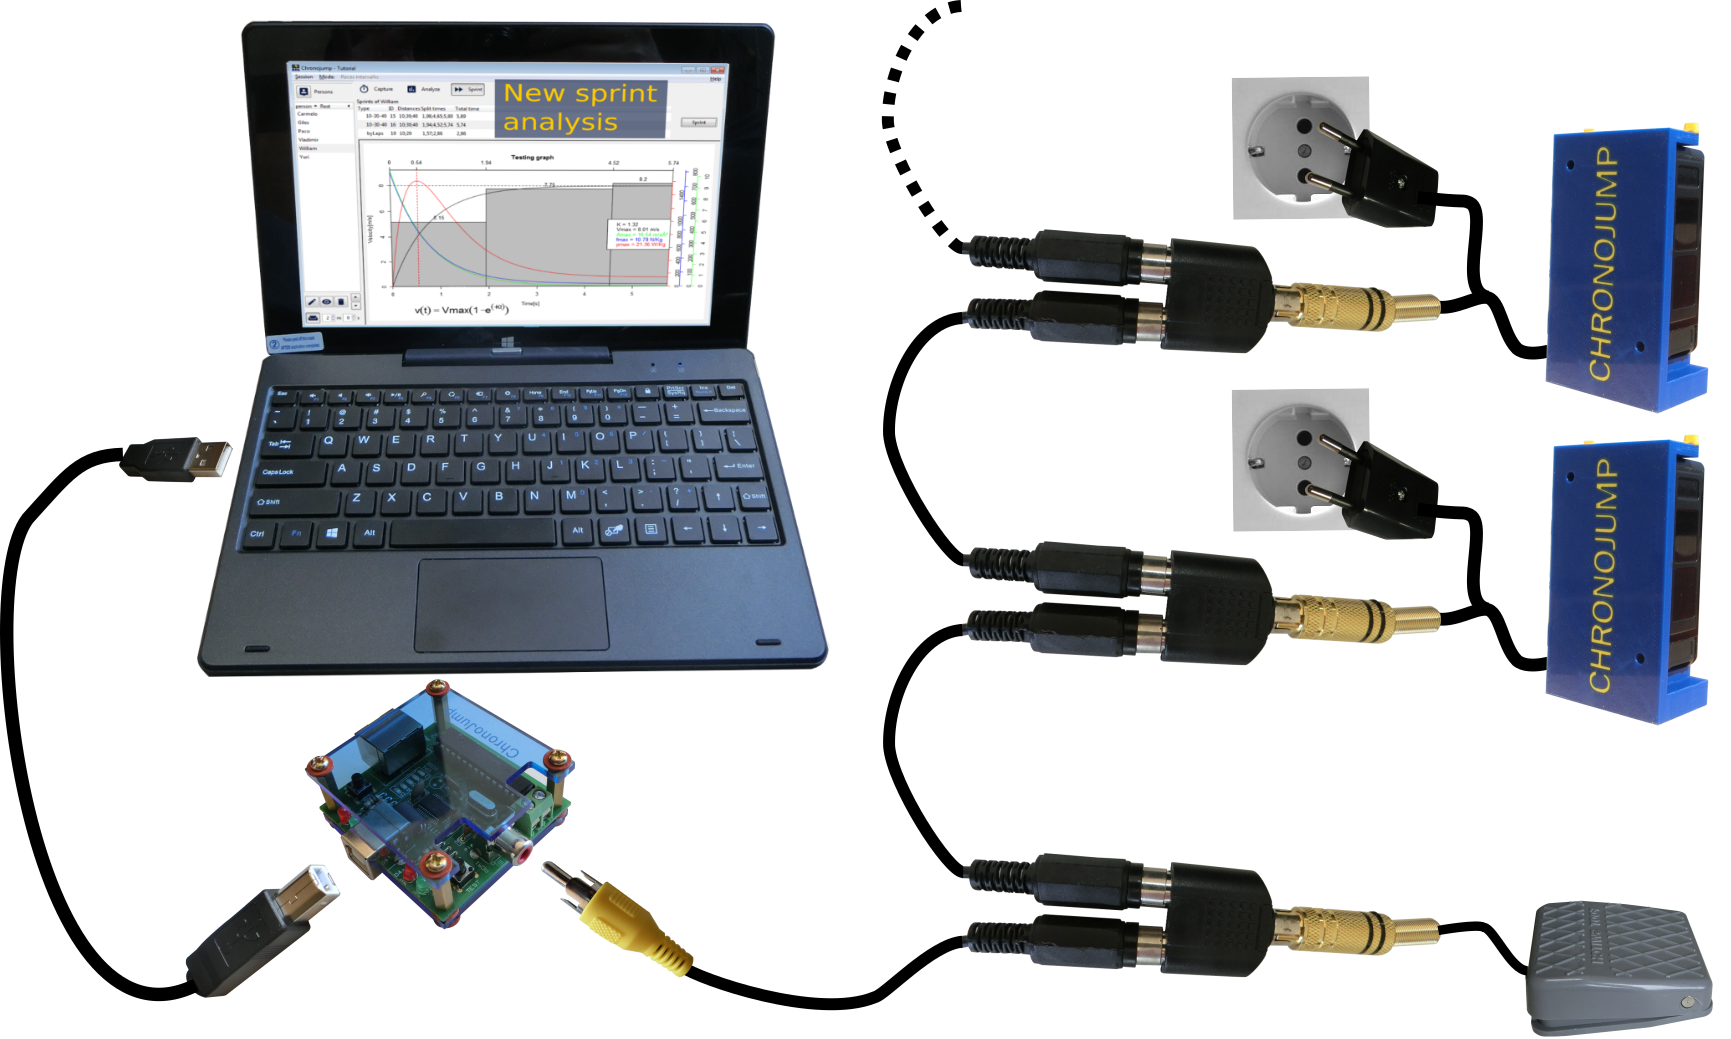
\includegraphics[width=0.6\columnwidth]{images/photocells-connections}
\par\end{centering}

\caption{\label{fig:Schem-two-photo}Drawing of two barriers and a switch to
measure races.}
\end{figure}


In order to calculate average speed, user will be asked about the
distance between platforms.

Runs can be of two types: simple and repetitive. On Chronojump a \textbf{simple
run} means that there's only one track. There are two kinds of \textbf{simple
runs}:
\begin{description}
\item [{Running~from~stop}] Start on contact in a device and end in contact
in the same or other device.
\item [{Running~with~initial~speed}] Start before the contact, after
a while, a contact is done and chronometer starts, then person leaves
the detection device until it produces contact again. This allows
to measure a run where person has an initial speed.
\end{description}
In both situations, the registered data is the time between one device
and the other, also speed will be calculated.

An \textbf{intervallic run} is a run where there's more than one track,
it should be understanded as ``run along two or more tracks limited
by devices at a fixed distance''.


\subsection{Raction time}

Chronojump allows to measure the reaction time. This time is the elapsed
time between a starting signal and the moment at which the subject
starts the movement.

To activate this option clic on ``Measure reaction time'' 
\includegraphics[scale=0.66]{images/reactTime}

The results will be shown in the tab ``Show table'' and the column``.

\begin{figure}[H]
\begin{centering}
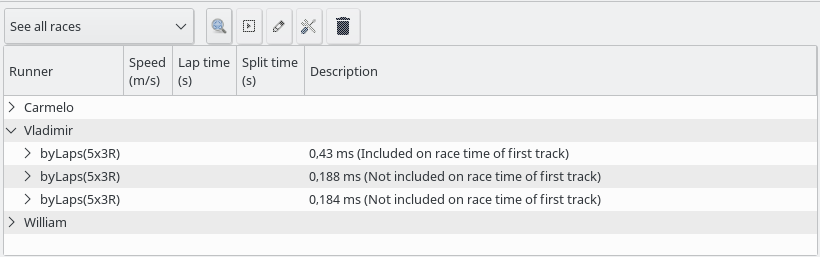
\includegraphics[scale=0.5]{images/races_Table}
\par\end{centering}

\caption{\selectlanguage{spanish}%
\label{fig:Races-table}\foreignlanguage{british}{Races results table}\selectlanguage{british}%
}
\end{figure}



\subsection{Correction of multiple contacts}

Chronojump allows to fix the situations where the subject activates
the contact device more than once due to different parts of the body
contact the device in different instants. (example: an athlete arrive
to a photocell, makes contact with a hand, ends the contact and after
that make contact with body).

To prevent this type of situations in Menu -> Preferences -> Runs
check \emph{Prevent double contacts}

\begin{figure}[h]
\begin{centering}
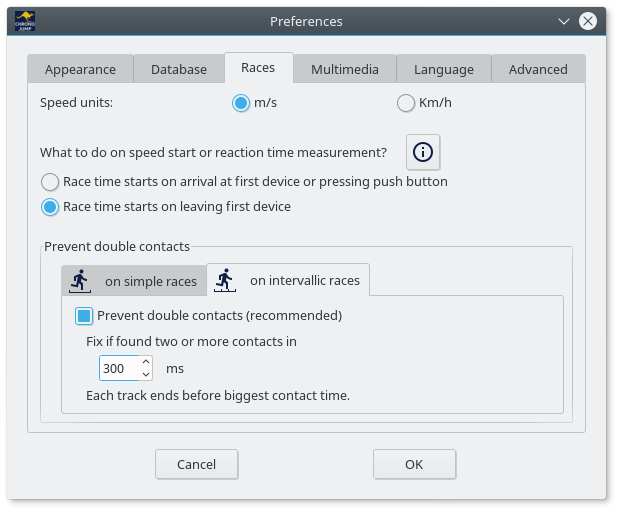
\includegraphics[scale=0.66]{images/preferences_double_contact}
\par\end{centering}

\caption{\selectlanguage{spanish}%
\label{fig:Double-contact}Double contact configuration\selectlanguage{british}%
}
\end{figure}


\noindent This dialog box allows to set the minimum time between contacts
to be considered as correct. If the time between contacts is lesser
than the configuration in the dialog Chronojump will consider the
instant when the longest contact start.

\noindent in the figure \ref{fig:Double-contact-example} is shown
an example of a race with multiple contacts situation.
\begin{figure}[H]
\begin{centering}
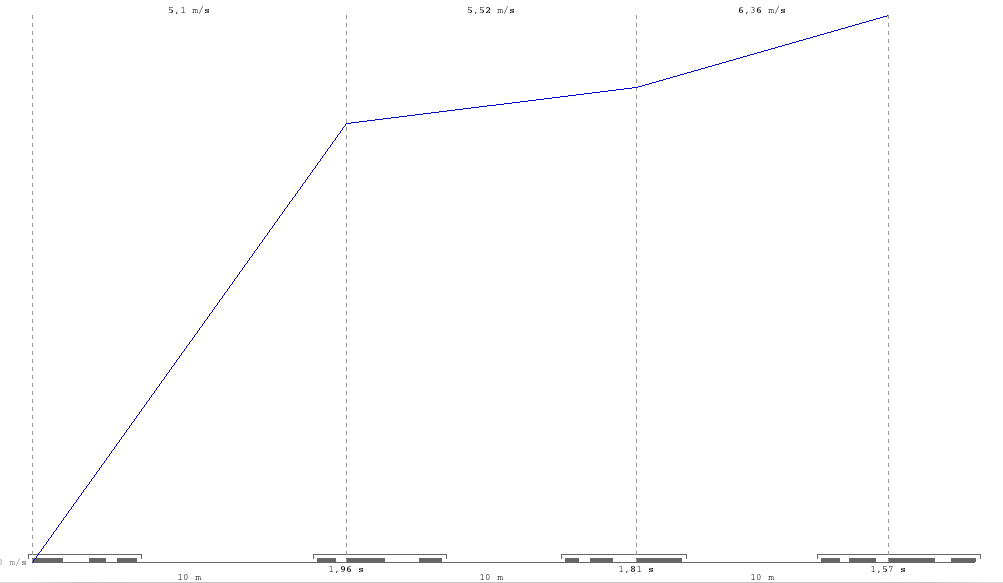
\includegraphics[scale=0.66]{images/races_double_contacts}
\par\end{centering}

\caption{\selectlanguage{spanish}%
\label{fig:Double-contact-example}\foreignlanguage{british}{Double
contacts example}\selectlanguage{british}%
}
\end{figure}


In the lower part of the graph, each real contact is shown as a segment
with a length equal to the duration of the contact. The segments are
grouped so that each cluster is treated as a single contact. The vertical
dashed lines show the instant when the start of the contact is considered.


\subsection{Simple races execution}

To execute a simple run, click the following buttons on\emph{ Runs}
tab:
\begin{itemize}
\item \emph{Custom} to run after introduce the track's distance
\item \emph{20m-400m}, to run on the preselected track's distance
\item Agility runs, this tests are available: 20 Yards, 505, Illinois, Shuttle
Run, Zig-Zag test. The figure \ref{fig:Test-de-agilidad-505} shows
the information available on software about the 505 test.
\end{itemize}
\begin{figure}[H]
\begin{centering}
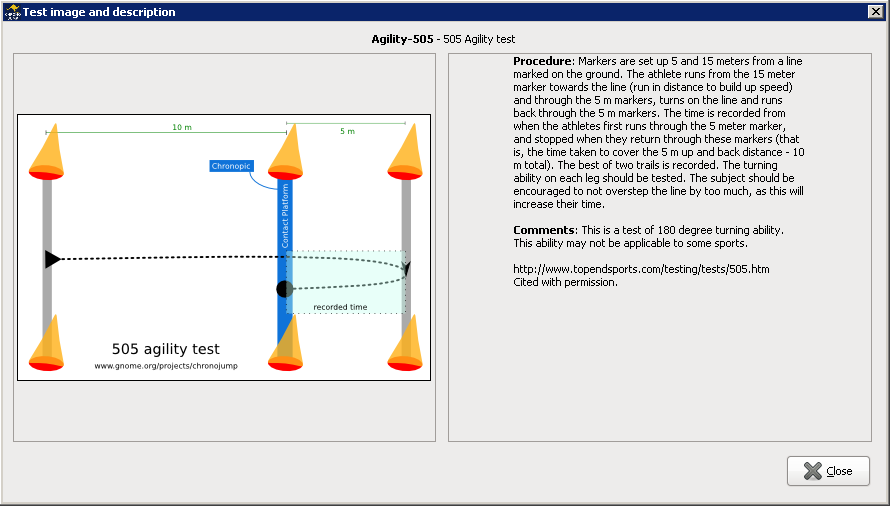
\includegraphics[scale=0.55]{images/chronojump-505}
\par\end{centering}

\caption{\label{fig:Test-de-agilidad-505}505 Agility test.}
\end{figure}


Click on \emph{More} to see all simple runs available, and execute
them clicking \emph{Ok}.

If Chronopic has not been connected and activated from Chronopic window,
a run will be simulated. In the other hand, if Chronopic is connected,
real run will be done. Software allows to start run in contact with
the device or before the contact. On the later situation, time between
starting of the run and contact on the first device is deleted.

In the pop-up window it shows the progress of the run, which may be
stopped by clicking on the \emph{Finish} or \emph{Cancel} button.

If you want to execute the same type of run to various subjects and
you don\textquoteright t want a button (only available on the tab
\emph{More}), you can change the subject and use the \emph{Last} button
to allow another person to perform the same run.


\subsection{Executing intervallic runs}

To execute an intervallic run, click the following buttons on \emph{Intervallic
Runs} tab:

\emph{By tracks}: intervallic run limited by number of tracks

\emph{By time}: intervallic run limited by number of tracks

\emph{Unlimited}: unlimited intervallic run

At som run types, user interaction will be needed, like track distance
and limit factor: tracks or seconds. Click on \emph{More} to get a
list of all the available of the intervallic runs and execute them
clicking OK. The run menu also provides access to these actions.

If Chronopic has not been connected and activated from Chronopic window,
a run will be simulated. In the other hand, if Chronopic is connected,
real run will be done. Software allows to start run in contact with
the device or before the contact. On the later situation, time between
starting of the run and contact on the first device is deleted.

In the pop-up window it shows the progress of the run, which may be
stopped by clicking on the \emph{Finish} or \emph{Cancel} button.

If you want to execute the same type of run to various subjects and
you don\textquoteright t want a button (only available on the tab
\emph{More}), you can change the subject and use the \emph{Last} button
to allow another person to perform the same run.


\subsection{Feedback auditive and visual at the intervallic runs: bells}

Similarly to the repetitive jumps, you can configure minimum and maximum
values dor each track. A red bell will be shown on a bad execution,
and a green bell on the opposite, also a distintive sound will be
played.

Configure this actions clicking on ``Bells''.


\subsection{Runs view}

Simple races are shown on the \emph{Races - Simple} mode and the intervallic
runs on the \emph{Races - intervallic} mode. In both cases, it\textquoteright s
included a filter for all the possible runs or only a particular type.

\begin{figure}[H]
\begin{centering}
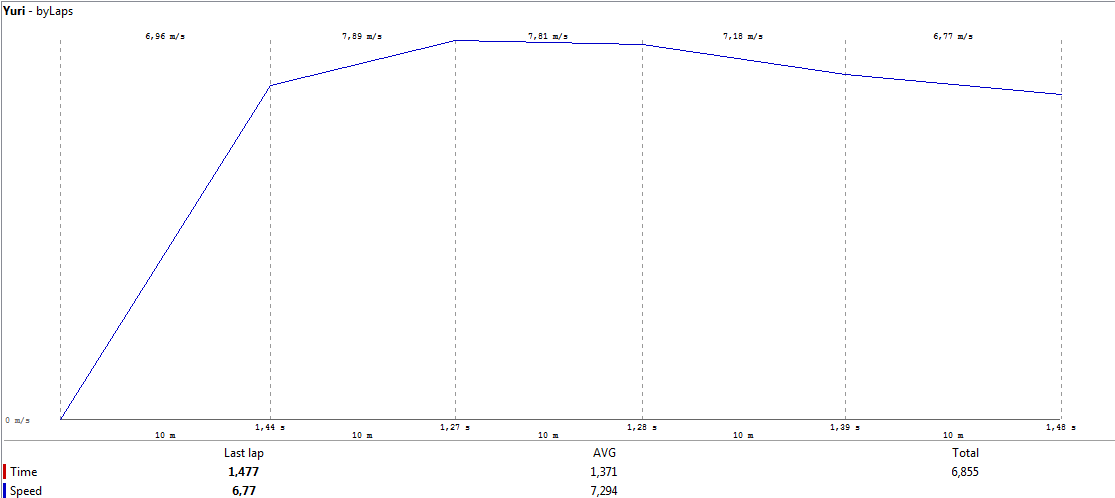
\includegraphics[scale=0.75]{images/race_graph}
\par\end{centering}

\caption{\selectlanguage{spanish}%
\label{fig:Race display}Lap race display\selectlanguage{british}%
}
\end{figure}


Tests are associated with the runners. The shown order of the tests
of each jumper is chronological so, the last test appears at the end
of the list. It\textquoteright s included a button that allows sorting
the tests by the type of run and not in chronological order. 

It\textquoteright s possible to change tests view by accessing at
the Preferences (more information in section \vref{sec:Preferencias}).

You can use the \emph{magnifying glass} button (or press \emph{z})
to facilitate the view of the tests.


\subsection{Runs edition}

You can add comments to a run or change the person (if you forgot
to change the current person previously) If you select the desired
run and click on the \emph{Edit} button on the selected run, you can
also find it on the menu, or by pressing the button \emph{e}.

In the intervallic runs, since they are composed of a set of runs,
this change will affect all the runs even if only one is selected.


\subsection{Repair intervallic runs}

Using \emph{Repair selected} button or pressing \emph{r}, you can
add a track, modify a time or delete a track. If an intervallic run
type has been defined to be limited to max \emph{n} tracks, or max
\emph{n} seconds, this conditions will limit the repair functionality.
When this happens, you will find an information text on the bottom
of the window.


\subsection{Runs delete}

To delete a run, select it and click the \emph{Delete selected run}
button. Its equivalent in the menu or press \emph{d} (delete). By
deleting the test you will be asked to confirm it if the delete confirmation
option is activated in the \emph{Preferences} menu (more information
in section \vref{sec:Preferencias}).

Deleting an intervallic run will delete all it's tracks.


\subsection{Creation of new run types}

In order to adapt the software to the needs of each user, it has been
included the function: \emph{Add run type} (on \emph{Runs} menu).
This allows trainer to define easily and powerully the desired run
types.

Created run type will be available on database to be used at any session,
and it will be listed clicking on the \emph{More} button at the \emph{Run}
or\emph{ Run intervallic} tabs (depending on which kind of run it's
created). This new run type will be also differentiated on statistics,
graphs and reports.

On creation, you should give it a distintive name and classify between
simple or intervallic. If run type is intervallic, then you can limit
is by tracks, time, or leave it unlimited.

The limit by tracks or time options can be defined as a fixed value
or leaved as undefined. If it's defined fixed, all new runs of this
type will be limited to that value; in the other hand, if the type
is not fixed, user will be asked by limit value everytime a new run
is done.

User can also fix the distances of the tracks. La ventana de creaci�n
de nuevo tipo de carrera concluye con la posibilidad de a�adir una
descripci�n textual. En las figura \ref{fig:Creaci=0000F3n-de-nuevo-tipo-carrera}
y \ref{fig:Creaci=0000F3n-de-nuevo-tipo-carrera-variable} puede observar
la ventana de creaci�n de nuevos tipos de carreras.

Last settings include: fix the distance of the tracks, and add a description
to the run type. In the figure \ref{fig:Creaci=0000F3n-de-nuevo-tipo-carrera}
you can see the creation of new run type.

\begin{figure}[H]
\begin{centering}
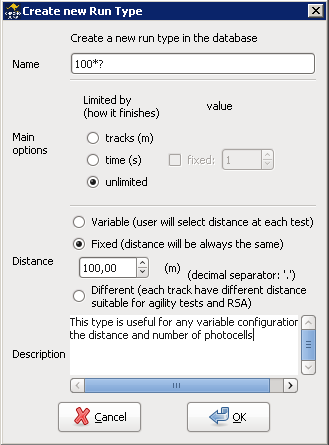
\includegraphics[scale=0.55]{images/run_type_add}
\par\end{centering}

\caption{\label{fig:Creaci=0000F3n-de-nuevo-tipo-carrera}Creation of a new
run type.}
\end{figure}


From Chronojump version 0.9, you can create intervallic runs with
variable track distance. This is suitable to calculate speed in the
different tracks of agility tests. In the test you can set the resting
time. 
\begin{figure}[H]
\begin{centering}
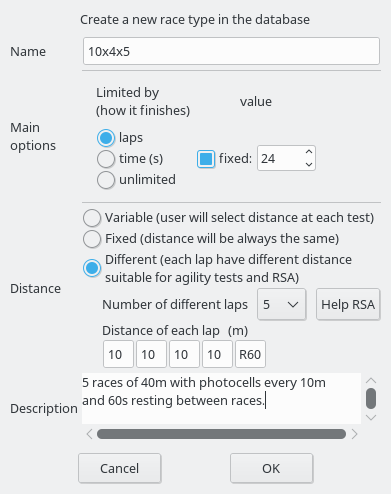
\includegraphics[scale=0.55]{images/run_type_add-variable}
\par\end{centering}

\caption{\label{fig:Creaci=0000F3n-de-nuevo-tipo-carrera-variable}Creation
of a new run type with variable tracks.}
\end{figure}



\subsubsection{Examples on creation of new run types}

Here you can find some examples on creating new run types. The names
of the types have been invented in this manual. The table \ref{tab:Ejemplos-de-tipos-carreras-creados}
is also useful to understand the different variables.
\begin{itemize}
\item \emph{``Sprint10''} 10 meters of sprint run.
\item \emph{``SprintShortVariable''} Run below 20 meters, each runner
will have run at a different distance defined by the trainer.
\item \emph{``20{*}5''} 100 meters run in 5 tracks of 20 meters.
\item \emph{``20{*}n''} 100 .Run 20{*}n meters (n tracks de 20 meters).
\item \emph{``40{*}50\%fatigue''} Intervallic run where each person runs
until 50\%fatigue is reached. Time needed to fatigue is individual
and known by trainer. Each track has 40m.
\item \emph{``100{*}?''} Person has to run tracks of 100m until trainer
(or runner) decides to finish.
\item \emph{``2 min of 20-10-7''} Agility run on 3 tracks that have to
be repeated during 2 minutes. First track has 20m, second 10m and
third 7m.
\end{itemize}
\begin{table}[H]
\begin{centering}
\begin{tabular}{|c|c|c|c|c|}
\hline 
Name & Type & Limited by & Fixed & Track length\tabularnewline
\hline 
\hline 
Sprint10 & Simple & - & - & Fixed(10)\tabularnewline
\hline 
SprintShortVariable & Simple & - & - & Variable\tabularnewline
\hline 
20{*}5 & Intervallic & Laps & Yes (5) & Fixed(20)\tabularnewline
\hline 
20{*}n & Intervallic & Laps & No & Fixed(20)\tabularnewline
\hline 
40{*}50\%fatigue & Intervallic & Time & No & Fixed(40)\tabularnewline
\hline 
100{*}? & Intervallic & Unlimited & - & Fixed(100)\tabularnewline
\hline 
2 min 20-10-7 & Intervallic & Time & Yes(120'') & Different(20,10,7)\tabularnewline
\hline 
10x4x5 & Intervallic & Laps & Yes(24){*} & Different(10,10,10,10,R60)\tabularnewline
\hline 
\end{tabular}
\par\end{centering}

\noindent \begin{centering}
{*}The last resting is not accounted. 24 = 5{*}4 + 4
\par\end{centering}

\caption{\label{tab:Ejemplos-de-tipos-carreras-creados}Examples on run types
created by user.}
\end{table}



\section{Encoder tests}


\subsection{Safety instruccions for linear encoders}

An encoder is a precise instrument that has to be managed ALWAYS with
care. Please follow this safety instructions.

If you broke your encoder contact us at hardware@chronojump.org


\subsubsection{Safety magnets}

Fix the encoder on iron or metal surface like the weights on a gym.
Note some gym weights are covered with rubber and have not magnet
power. 
\begin{figure}[H]
\noindent \begin{centering}
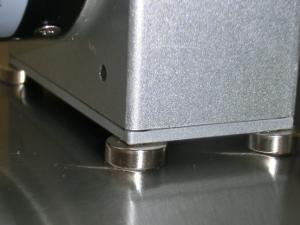
\includegraphics{images/encoder-manual-images/magnets.jpeg}
\par\end{centering}

\caption{Magnets on a metal surface}
\end{figure}



\subsubsection{Do not release}

Do not release the wire when it is extended because it will return
at high speed and will break it.

\begin{figure}[H]
\noindent \begin{centering}
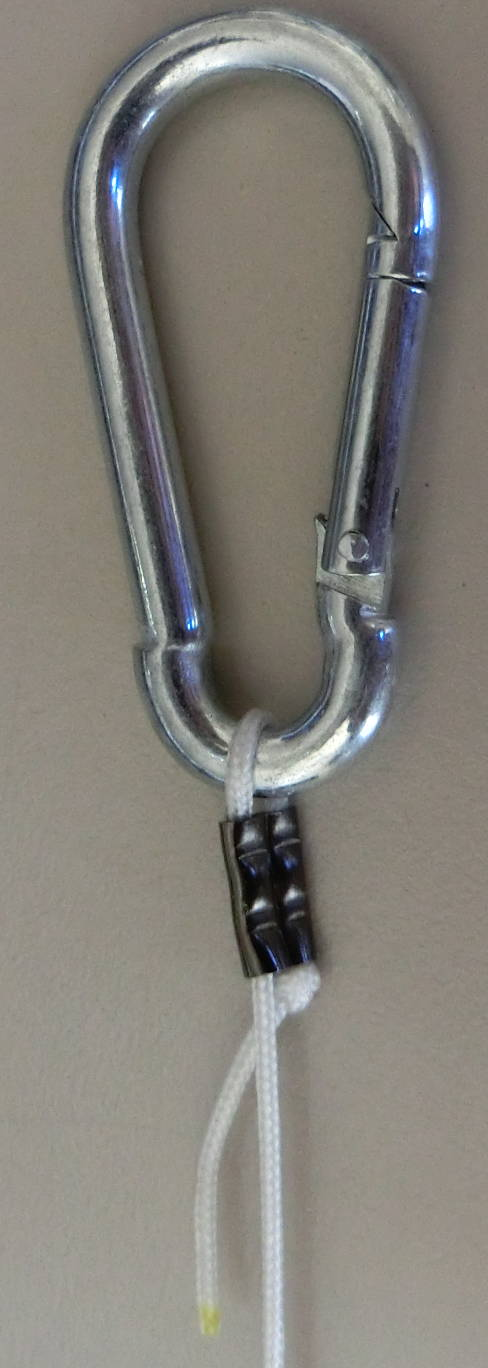
\includegraphics[scale=0.25]{images/encoder-manual-images/handle.jpeg}
\par\end{centering}

\caption{Wire handle}
\end{figure}



\subsubsection{Make sure that the cable is correctly fixed}

Allways be careful when manipulating the carabiner. Ensure that it
is well secured in your fingers. A wrong grab could end up with a
broken encoder. When possible, try to put a finger inside the carabiner
to avoid it slipping from your fingers.

\begin{figure}[H]
\noindent \begin{centering}
\begin{tabular}{|c|c|}
\hline 
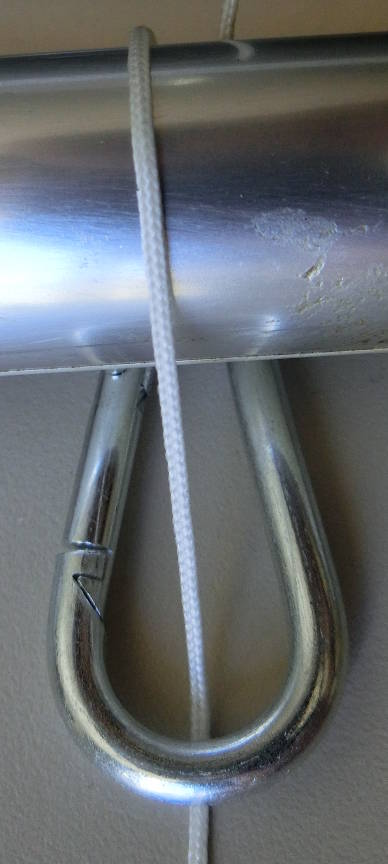
\includegraphics[scale=0.5]{images/encoder-manual-images/attachedEncoder.JPG} & \includegraphics[scale=0.5]{images/encoder-manual-images/encoderOnPlates.JPG}\tabularnewline
\hline 
\hline 
Fixing on a barbell & Fixing on a plates loads\tabularnewline
\hline 
\end{tabular}
\par\end{centering}

\caption{examples of fixing}
\end{figure}



\subsubsection{Do not exceed the 2.5m of range of movement}

The encoder cable is 3m long but it never must be fully extended.

Remember that this limitation refers to the range of movement. If
necessary, you can lengthen the thread by attaching another thread
to the encoder.


\subsubsection{Perpendicular use}

Perpendicular use: Encoder measures distance, speed and power of the
wire assuming it's perpendicular to the surface. If you pull/push
the wire with an inclination, data will not be accurate and the wire
can be damaged. 

\selectlanguage{spanish}%
\begin{figure}[H]
\selectlanguage{british}%
\noindent \begin{centering}
\begin{tabular}{|c|c|c|c|}
\hline 
\includegraphics[scale=0.25]{/home/xpadulles/chronojump-docs/images/encoder-manual-images/encoderWrong1} & \includegraphics[scale=0.25]{/home/xpadulles/chronojump-docs/images/encoder-manual-images/encoderWrong2} & \includegraphics[scale=0.25]{/home/xpadulles/chronojump-docs/images/encoder-manual-images/encoderCorrect1} & \includegraphics[scale=0.25]{/home/xpadulles/chronojump-docs/images/encoder-manual-images/encoderCorrect2}\tabularnewline
\hline 
\hline 
Wrong & Wrong & Right & Right\tabularnewline
\hline 
\end{tabular}
\par\end{centering}

\caption{Examples of wrong and right using of the encoder}
\selectlanguage{spanish}%
\end{figure}


\selectlanguage{british}%

\subsection{Concepts}

This manual briefly describes some concepts. Understanding them is
important to use the software appropriately.


\subsubsection{Database}

Chronojump stores data in one database file. Thus, instead of collecting
the information in individual files for each session, most of the
information is organized in a single file to facilitate the study
of relationships between:
\begin{itemize}
\item sessions
\item subjects
\item exercises
\item repetitions
\end{itemize}
All modifications in session, subjects and exercises, will be updated
at any time in the database. So there isn\textquoteright t need to
save the information periodically. If rare case, the program crash,
you wouldn\textquoteright t lose any data except sometimes the exercise
that is being performed at the time.


\subsubsection{Sessions}

The sessions represent situations where the coach or evaluator gathers
subjects for a series of tests. Every time you gather a group of athletes
to be tested in a short space of time (usually one day), you should
create a new session. Although the subjects to assess can be the same
as in other session, you should create a new one and load them from
the other session. In this way, you can make comparisons between data
over time.


\subsubsection{subjects}

All individuals able to perform the tests are known as subjects. It\textquoteright s
strongly recommended to create one person only once in order to study
the evolution over time. In following sessions the person can be loaded.


\subsubsection{Exercices}

Every time you want to measure, you perform an exercise. Exercise
has a name (e.g. Bench press), an extra weight (e.g. 40Kg), type of
contraction (e.g. concentric), laterality (e.g. both limbs), recording
time (e.g. 45s) and others.


\subsubsection{Sets (formerly signals)}

When the person does the exercise, encoder generates a lot of data
and sends it to the computer. Exercise duration is defined by the
user who manages the software, but can be shortened if wanted. All
the data received is called a \textquotedblleft set\textquotedblright .
This set is saved automatically when capture ends. The set is meaningless,
it doesn't have any information on how many repetitions of the movement
has been done by the person who executed the exercise.


\subsubsection{Repetitions (formerly curves)}

When set is analysed, a number of repetitions are found. This repetitions
have the mechanical data wanted by the evaluator: start, duration,
speed, force, power. The repetitions are detected by the software
automatically following user criteria. Videotutorial: Saving Repetitions
\url{https://youtu.be/MoFKMGGLbdw}


\subsection{Using the encoder}

Chronojump main windows

\begin{figure}[H]
\noindent \begin{centering}
\includegraphics[scale=0.5]{images/encoder-manual-images/main}
\par\end{centering}

\caption{Main window}
\end{figure}


A) Starting on the top left of main window, there's a menu bar with
session options and help. You should start your work creating a new
session or loading an existing one.

B) The rest of the left part of the screen is related to subjects.
On the top you can create new subjects or load from another session.
Below you can select the current person and finally, at the bottom
you can edit the person, see all it's tests and delete it.

C) The centre-right part of the screen is for managing the tests (or
exercises). At the top there are two tabs: contacts and encoder. Select
the encoder tab.

Inside the capture area there's six different areas

\begin{figure}[H]


\noindent \begin{centering}
\includegraphics[scale=0.5]{images/encoder-manual-images/capture_area}\caption{Capture area}

\par\end{centering}

\end{figure}



\subsubsection{Set configuration}

This area shows the configuration of the set (machine used, exercise
typo of contraction, laterality and load)

Clicking on the set configuration button will expand the corresponding
dialog.

\begin{figure}[H]
\noindent \begin{centering}
\includegraphics[scale=0.75]{images/encoder-manual-images/set_config_button}
\par\end{centering}

\caption{Set config button}
\end{figure}


This will expand the set configuration dialog.

\begin{figure}[H]
\noindent \begin{centering}
\includegraphics[scale=0.5]{images/encoder-manual-images/set_config}
\par\end{centering}

\caption{Set configuration}
\end{figure}



\subsubsection{Encoder configuration}

The first step for configuring the set consists in selecting the type
of encoder connected, the type of machine at which the encoder is
connected and the exercise that will be performed.

\begin{figure}[H]
\noindent \begin{centering}
\includegraphics[scale=0.75]{/home/xpadulles/chronojump-docs/images/encoder-manual-images/select}
\par\end{centering}

\caption{Encoder config button}
\end{figure}


Clicking on \emph{Configure} button will show a new windows with different
combinations of encoders/machines. Each type of encoder has a different
set of configurations. The arrow buttons allow to change between different
configuration of each encoder.

In 1.7.0 and newer versiona Chronojump can manage multiple encoder
config. This way you can Create, delete, import and export diferent
encoder configuration.

\begin{figure}[H]
\noindent \begin{centering}
\includegraphics[scale=0.5]{images/encoder-manual-images/encoder_admin}
\par\end{centering}

\caption{Encoder configuration admin}
\end{figure}


Each type of encoder has a diferent set of configurations. Clicking
on the arrow buttons will change the configuration for this type of
encoder.

There are three types of encoder:
\begin{itemize}
\item Linear.
\item Rotary friction.
\item Rotary axis.
\end{itemize}
Some configurations need additional parameters as angle, diameter
or inertia momentum. Videotutorial: Capturing on an inclined plane
machine \url{https://youtu.be/s-8Zel1RtGs}


\paragraph{Inertial machines configuration}

The characteristics of the inertial machines make necessary to enter
a set of extra parameters that are being descrived below:
\begin{figure}[H]
\noindent \begin{centering}
\includegraphics[scale=0.5]{/home/xpadulles/chronojump-docs/images/encoder-manual-images/inertial_conf}
\par\end{centering}

\caption{Inertial machines parameters}
\end{figure}


Using the rotary axis encoder (the most common), there's four types
of intertial machines configuration depending on whether its movement
is vertical or horizontal and wether the force is applied directly
on a rope/ribbon or the force is applied on a moving pulley:

\selectlanguage{spanish}%
\begin{figure}[H]
\noindent \centering{}%
\begin{tabular}{|c|c|c|}
\cline{2-3} 
\multicolumn{1}{c|}{\selectlanguage{british}%
\selectlanguage{spanish}%
} & \selectlanguage{british}%
Without moving pulley\selectlanguage{spanish}%
 & \selectlanguage{british}%
With moving pulley\selectlanguage{spanish}%
\tabularnewline
\hline 
\selectlanguage{british}%
Vertical\selectlanguage{spanish}%
 & \includegraphics[scale=0.5]{/home/xpadulles/chronojump-docs/images/encoder-manual-images/InertialMachine-01} & \includegraphics[scale=0.5]{/home/xpadulles/chronojump-docs/images/encoder-manual-images/InertialMachine-03}\tabularnewline
\hline 
\selectlanguage{british}%
Horizontal\selectlanguage{spanish}%
 & \includegraphics[scale=0.5]{/home/xpadulles/chronojump-docs/images/encoder-manual-images/InertialMachine-02} & \includegraphics[scale=0.5]{/home/xpadulles/chronojump-docs/images/encoder-manual-images/InertialMachine-04}\tabularnewline
\hline 
\end{tabular}\caption{\selectlanguage{british}%
Rotary axis encoder configuration\selectlanguage{spanish}%
}
\end{figure}


\selectlanguage{british}%
Below are descrived the needed parameters:
\begin{itemize}
\item Number of anchorages: Some models of inertial machines have more than
one anchorage allowing to change the mean diameter where the rope
is wrapped. Selecting the number of anchorages will add or supress
the options to enter the diameter of each one.
\item Inertia momentum: This is a parameter that depends on each machine
and is reffered to the machine without any extra load. Chronojump
implements a system to calculate the inertia momentum that allows
to config an encoder in almost all type of inertial machines. Follow
the instructions in section \index{5.3.3.2.2} to calcuate the inertia
momentum of your machine configuration.
\item Mass of each extra load: If the inertial machine allows to add extra
loads to augment the inertia momentum, Chronojump will calcule it
from the mass of eache one of this loads. This way, you have to enter
the mass o only one load.
\item Distance center-load: It is the distance between the center of the
extra load and the axis of the inertial machine.
\item Force multiplier factor: This parameter especifies the configuration
of the pulleys set that allows the resistance of the machine to be
a multiple or a fraction of the force that the machine would offer
without the pulleys set.
\end{itemize}

\subparagraph{Calculation of the inertia momentum}

The firs part of this section will explain how to calculate the inertia
momentum (IM) of the disk in an inertial machine. The calculus of
the IM of a disk with attached weights will be discussed in the second
part. In the following link you can see a video of the process.

\href{http://youtu.be/HK1ilOyg5Vs}{Calculing inertia momentum video}


\subparagraph{Inertia momentum of the disk}

To calculate the IM of the bare disk without weights we will use a
reference weight. Remember, although we will use an attached to the
disk weight, the results given by Chronojump in this part of the process
refers only to the disk without any weight.
\begin{enumerate}
\item Put the machine in a any position that makes the disk rests in a vertical
plane.
\item Attach a known weight to known distance from the center of the disk.
This way the disk will be unbalanced and after lifting and living
the weight it will start to oscilate like a pendulus.
\begin{figure}[H]
\noindent \centering{}\includegraphics[scale=0.06]{images/encoder-manual-images/Disk}\caption{Reference weight}
\end{figure}

\item In chrono jump software, with the encoder connected go to Select encoder.
\begin{figure}[H]
\noindent \begin{centering}
\includegraphics{images/encoder-manual-images/select}
\par\end{centering}

\caption{Select encoder button}
\end{figure}

\item Choose type of encoder you will use, and select the Inertial machine
option.
\item In this windows you will be asked for the diameter where the rope
is wrapped and the IM of the machine. Note that in conical machines
this diameter changes continuously as the disk is spinning. We recommend
you to use the mean diameter of the part of the cone where the rope
is wrapping at. 
\begin{figure}[H]
\noindent \begin{centering}
\includegraphics[scale=0.5]{images/encoder-manual-images/inertial_conf}
\par\end{centering}

\caption{Parameters of the inertial machine}
\end{figure}

\item As you want to know the IM, click on \textquotedblleft Calculate IM\textquotedblright{}
\item Enter the weight (in grams) of the reference load and the distance
(in centimeters) to the center of the disk.
\begin{figure}[H]
\noindent \centering{}\includegraphics[scale=0.5]{images/encoder-manual-images/calculus}\caption{Parameters for calculating the IM}
\end{figure}

\item Pull the weight to approximately 90 degrees position and leave it.
The disk should start swinging.
\item Quickly, click on the capture button. You will see the signal sent
by the encoder. Chrnonojump will detect when the machine stops moving
and will return the calculated IM.
\begin{figure}[H]
\noindent \centering{}\includegraphics[scale=0.33]{images/encoder-manual-images/oscilation}\caption{Capturing the oscilation}
\end{figure}

\end{enumerate}

\subparagraph{Inertia momentum of the disk with attached weights.}

In the encoder configuration you should enter the distance from the
center of the extra loads to the axis of the disk as well as the weight
of the extra weights. This way in the exercise capture windows you
will be asked for the extra weights that are attached to the disk
as shown in the figure below.

\begin{figure}[H]
\noindent \centering{}\includegraphics[scale=0.75]{images/encoder-manual-images/capture_inertial}\caption{Exercise capturing with inertial configuration}
\end{figure}


Below the extra loads selection box the total inertial momentum is
shown in Kg{*}cm\texttwosuperior{}

Chronojump uses the next formulae:

$I_{w}=M*d^{2}$

Where:
\begin{itemize}
\item $I_{w}$ is the Inertia momentum that each weigth will add to the
system.
\item $M$ is the mass of the weight.
\item $d^{2}$ is the square of the distance from the center of the disk
to the center of the weight.
\end{itemize}
And the inertia momentum of the disk with the attatched weights

$I=I_{d}+n*I_{w}$

Where:

$I$ is the total inertia momentum. This is the value you must enter
in the chronojump software.

$I_{d}$ is the inertia momentum of the disk calculated in the first
part of this section.

$n$ is the number of weights added to the disk. - is the inertia
momentum of each weight calculated above


\subsubsection{Exercise configuration}

In the exersise section you will find a drop-down with some preconfigured
exercises. Chronojump allows to edit an exercise \includegraphics[scale=0.75]{/home/xpadulles/chronojump-docs/images/edit_button}
or create a new one \includegraphics[scale=0.75]{/home/xpadulles/chronojump-docs/images/create_button}.\foreignlanguage{spanish}{}
\begin{figure}[h]
\selectlanguage{spanish}%
\noindent \centering{}\includegraphics[scale=0.75]{/home/xpadulles/chronojump-docs/images/encoder-manual-images/exercise_window}\caption{\selectlanguage{british}%
Exercise configuration window\selectlanguage{spanish}%
}
\selectlanguage{british}%
\end{figure}


In the exercise configuration window the following parameters will
be shown:
\begin{itemize}
\item Name of the exercise: Identifying text that will be shown in the exercise
drop-down.
\item Displaced body weight: Percentage of the body that is displaced during
the exercise.
\item Resistance: Descriptive text where is specified the type of resistance
used.
\item Description: Short information text with the description of the exercise.
\item Speed at 1RM: Speed of execution when the load is the one that allows
to only one repetition. This parameter is mandatory if you want to
calculate the 1RM with the method ``1RM any exercise''.
\end{itemize}

\subsubsection{Selection of phase or phases analysed}

At the time of showing or analyzing you must select if the concentric
phase (force in the same way that speed) \includegraphics[scale=0.5]{images/encoder-manual-images/concentric}
or both (excentric and concentric) \includegraphics[scale=0.5]{images/encoder-manual-images/eccentric_concentric}.


\subsubsection{Laterality}

For information purpouses the laterality with which is executed the
exercise is also stored. This will be usefull is you want to see asymmetries
in different muscle groups.


\subsubsection{Resistance}

Finally, the resistance that will be used is configured.

In the gravitatory exercises. the extra mass that will be moved will
be introduced without taking in account the mass of the athlete.

\begin{figure}[H]


\noindent \begin{centering}
\includegraphics[scale=0.75]{images/encoder-manual-images/mass_config}\caption{Configuring the extra mass}

\par\end{centering}

\end{figure}


The extra mass of the exercise will be calculated using the formula

\selectlanguage{spanish}%
\[
TotalMass=\frac{PersonMass*\%DisplacedBodyWeight}{100}+ExtraMass
\]


\selectlanguage{british}%
At the right of the total mass will be shown at which percentage of
the 1RM of the person the extra mass corresponds.

In the case of inertial exercises, the diameter (depending on the
ancorages) and the extra loads need to be entered.

\begin{figure}[H]


\noindent \centering{}\includegraphics[scale=0.75]{images/encoder-manual-images/inertia_config}\caption{Inertia config}
\end{figure}



\subsection{Capture configuration}

In the acquire area a new set can be captured \includegraphics[scale=0.5]{images/capture_button}
or a previusly captured one can be loaded \includegraphics[scale=0.75]{images/load_signal_button}.

\shadowbox{\begin{minipage}[t]{1\columnwidth}%
Important!: Using inertial machines, after opening the software the
first time that an aquisition is made, a calibration of the machine
must be done. It requires to unwrap completely the rope/ribbon and
clicking on calibrate.

\noindent \begin{center}
\includegraphics[scale=0.5]{images/encoder-manual-images/inertial_calibration}
\par\end{center}

When using inertial machiens, remember always start with the rope
fully unwrapped when you press the capture button. I you don't do
that, you will see that half of the repetitions have a much smaller
range of movement than the other half.

\noindent \begin{center}
\begin{tabular}{|c|c|}
\hline 
Right execution & Wrong execution\tabularnewline
\hline 
\hline 
\includegraphics[scale=0.25]{images/encoder-manual-images/inertial_right} & \includegraphics[scale=0.25]{images/encoder-manual-images/inertial_wrong}\tabularnewline
\hline 
\end{tabular}
\par\end{center}%
\end{minipage}}

During the capturing process you can finish \includegraphics[scale=0.5]{/home/xpadulles/chronojump-docs/images/encoder-manual-images/finish_button}
or cancel \includegraphics[scale=0.5]{/home/xpadulles/chronojump-docs/images/encoder-manual-images/cancel_button}
the set. In the first case the capture will finish and the data will
be saved. In the second case the data will be discarded as well as
all the associated data.


\subsubsection*{Feedback /Rhythm}

This window shows the information that will be shown during the capturing
process.

\begin{figure}[H]
\noindent \centering{}\includegraphics[scale=0.5]{images/encoder-manual-images/bells}\caption{\label{fig:Feedback}Feedback options}
\end{figure}


In the Feedback tab you can configure the visual and sound signals
in function of the selected variable and referred to the best repetition
or to the history of the athlete with this load and exercise.

The drop-down allows to select the variable that will be used to colour
in green, blue or red each repetition.

The bells allow to config the threshold at which the bars will be
shown in green (greater than the specified value) or red (less than
the specified value)

\noindent \begin{flushleft}
The Rhythm tab allows to configure an advanced metronome in which
you can select the desired time of each phase of the execution.\begin{wrapfigure}{l}{0.5\columnwidth}%
\noindent \centering{}\includegraphics[scale=0.5]{images/encoder-manual-images/rhythm}\caption{\label{fig:Rhythm}Rhythm}
\end{wrapfigure}%

\par\end{flushleft}

Selecting \emph{Show rhythm while capturing} will show a set of options
that will allow to config the duration of the excentric and concentric
phase.

If you want to use cluster of sets, click on \emph{Use clusters.}
This option allows to execute the specified number of repetitions
in a cluster and rest the amount of seconds specified between clusteres.


\subsubsection*{Load}

The load button \includegraphics[scale=0.75]{images/load_signal_button}
of this frame allows to load a set, save set again with a comment
(just write comment in the area and press update), or delete the set.
The load set window is used also to manage all the sets of current
person. Right click on it to change the person who performed the exercise,
add a comment or delete any set of a given person. Videoturotial:
Edit set \url{https://youtu.be/UiZJKbU4OSg}


\subsubsection*{Recalculate}

Recalculate can be used after capturing or loading. When user detects
that some parameter has not been set correctly and wants to perform
calculations of the set again, user can change the selector and press
\textquotedblleft recalculate\textquotedblright{} \includegraphics[scale=0.75]{images/recalculate}.
E.g. 40 seconds squat has been done and the extra weight introduced
was 40Kg but user forgot to add the weight of the lift bar. After
capture, user can change 40Kg to 55Kg and then press \textquotedblright recalculate\textquotedblright{}
in order to have the force and power calculated correctly.


\subsubsection*{Delete}

If you need to delete a set, click on the trash icon \includegraphics[scale=0.75]{/home/xpadulles/chronojump-docs/images/encoder-manual-images/delete_set}.


\subsection{Chronopic}

The device button allows to specify which typo of device is going
to be used. Each time a new device is connected to Chronojump the
type of device must be specified. This configuration will be remembered
by Chronojump for future uses.

\begin{figure}[H]


\noindent \begin{centering}
\begin{tabular}{|c|c|}
\hline 
Chronopic not configured & Chronopic configured\tabularnewline
\hline 
\hline 
\includegraphics[scale=0.5]{images/device_window} & \includegraphics[scale=0.5]{images/encoder-manual-images/device_window_encoder}\tabularnewline
\hline 
\end{tabular}\caption{Device window}

\par\end{centering}

\end{figure}



\subsection{Bars of the main variable}

The bars frame shows, during the exercise, the main variable in real
time. This way the athlete can have an instant feedback of every execution
of the exersice.

\begin{figure}[H]
\noindent \begin{centering}
\includegraphics[scale=0.5]{images/encoder-manual-images/power_bars}
\par\end{centering}

\caption{Power bars}
\end{figure}


The descending white line in the bar indicates an excentric repetition.
An ascending line, a concentric.

The saved repetitions apears with a framed number below.


\subsection{Repetitions table}

Once set is loaded, captured or recalculated, Chronojump will find
repetitions and write their data on a table. Here you can delete a
repetition, save the selected repetition, save all or export them
to an spreadsheet software. Most users will save only a repetition,
or delete a repetition and the press \textquotedblleft save all\textquotedblright .
This repetitions can be analysed at the Encoder analyse tab.

\begin{figure}[H]
\noindent \begin{centering}
\includegraphics[scale=0.7]{images/encoder-manual-images/save_curve}
\par\end{centering}

\caption{Saving and deleting repetitions}
\end{figure}


To save or delete a repetition just click on the checkbox ``Saved''
of the repetition you want to save or delete.

In excentric-concentric mode, saving a excentreic (concentric) repetition
will also save the corresponding concentric (excentric) repetition
of the exercise.


\subsection{Raw data}

During the capture this frame will show the set sent by the encoder.
Once finished Chronojump will calculate all the repetitions and show
them in the same frame with some basic graphic information.


\subsection{Encoder settings and preferences}

In order to configure the encoder capture parameter, in \textquotedblleft Menu
-> Session -> Preferences -> Encoder capture\textquotedblright{} you
will find the next parameters:



\begin{figure}[H]
\noindent \begin{centering}
\includegraphics[scale=0.5]{images/encoder-manual-images/encoder_capture_preferences}\caption{Encoder preferences}

\par\end{centering}

\end{figure}

\begin{itemize}
\item Recording time. Sets how long Chronojump will register during the
set in case the capture is not cancelled manually.
\item End at n inactivity seconds. If Chronojump detects that the encoder
is not measuring any movement during this seconds, the program will
finish the capture process.
\item Minimal height. The minimum range of movement of a repetition in centimeters.
For example, in a bench press taking the bar for the first time (from
a bar support) won't be considered as a repetition because the rang
of movement is less than the value specified.
\item (Inertial) On inertial discard first repetitions: Allows to discard
the submaximum repetitions in whitch the subject has not reached the
maximum velocity of execution. This repetition will not be taken in
account when calculing the mean values of the set and will be drawn
in gray.
\item Show only bars. This option allows that the repetitions table to be
shown in another table and not show the raw data area, reserving much
more space for the bars area. To see the repetitions table click on
the tab ``table'' in the left lower part of the area.
\begin{figure}[H]


\noindent \begin{centering}
\begin{tabular}{|c|c|}
\hline 
Normal configuration & Only bars configuration\tabularnewline
\hline 
\hline 
\includegraphics[scale=0.25]{images/encoder-manual-images/no_only_bars} & \includegraphics[scale=0.25]{images/encoder-manual-images/only_bars}\tabularnewline
\hline 
\end{tabular}\caption{Only bars option}

\par\end{centering}

\end{figure}


\begin{itemize}
\item Show all bars. If this option is selected all the repetitions will
be shown and after each repetition all the bars will be resized to
fit in the bars area.
\item Show only last n bars. Allows to show only the last bars of the set.
In this mode the bars won't be resized but at each repetition the
bars wil slide from right to left.
\end{itemize}
\item Save repetitions automatically. Allows to save the repetitions automatically
depending on the specified criterion.
\item Cut sets into repetitions using triggers. In the section \index{5.3.11}
the use of the triggers during the set is detailed.
\end{itemize}

\subsection{Other encoder configurations}

In the tab called ``Encoder other'' some preferences that are less
commonly used can be found.
\begin{itemize}
\item If you want to do calculations of mechanical parameters only in the
propulsive phase just ensure the parameter \textquotedblleft propulsive\textquotedblright{}
is active. The meaning is the following: In a fast concentric movement
where there's little weight displaced, the brake action of the person
in the final phase of the movement will not be used in the calculations.
Nowadays most coaches prefer this option active because they noticed
that the comparison of mean power between a light weight and a heavy
weight exercise is not fair because the brake phase in the light weight
exercise is related to negative force and the power values get very
low. Then, if \textquotedblleft propulsive\textquotedblright{} phase
is active, only this is used, and not the \textquotedblleft brake\textquotedblright{}
phase.
\item The next options are related to smoothing of the capture and we recommend
to leave them untouched.
\item In the \emph{1RM prediction,} the method to get the linear regression
can be selected. The exponent in the weight means that the larger
is the mass of the point used the larger is the weight used for the
regression. The function of the weight can be zero (non wighted),
one (linear), two (quadratic) or three (cubic).
\end{itemize}

\subsection{Using triggers}

\begin{wrapfigure}{o}{0.5\columnwidth}%


\noindent \begin{centering}
\includegraphics[scale=0.25]{images/PushButton}\caption{Push Button}

\par\end{centering}

\end{wrapfigure}%


Since 2017, the Chronopic new models allows to read external synchronization
signals or triggers. These signals will be generated using any device
that close an electric contact (button, photocell, contact platform...).
You can check if your Chronopic can read it by pressing the test button
in it. If a green LED turns on it means that your device can receive
trigger signals.

These signals can be used to cut the set into repetitions so that
each signal indicates the start of a repetition or simply to highlight
an instant that could be of interest. To specify this behavior go
to Menu -> Session -> Preferences -> Encoder -> Cut sets into repetitions
using triggers.

If you want to identify certain instants inside the execution of the
exercise, in the instantaneous analysis of the repetition you will
see a dashed vertical yellow line that indicates the moment at which
was produced the trigger signal.

\selectlanguage{spanish}%
\noindent \begin{center}
\begin{figure}[H]
\noindent \centering{}\includegraphics[scale=0.33]{/home/xpadulles/chronojump-docs/images/encoder-manual-images/trigger}\caption{\selectlanguage{british}%
\label{tab:Triggers}Triggers\selectlanguage{spanish}%
}
\end{figure}

\par\end{center}

\selectlanguage{british}%
Besides, if you want to se the instants in milliseconds of the rising
(In) and falling (Out) flank you can click on the tab ``Show triggers''
on the lower side of the analysis frame.


\subsection{Examples of encoder use}

At the Gym: 
\begin{enumerate}
\item On the floor, at the side of the weight bar, put a gym weight (not
made by rubber) and encoder on the top of it (attached with the magnets).
\item The carabiner is attached to the barbell or the training machine.
\item Athlete1 and athlete2 start the warming up slowly and full range of
movement (in a different place) while evaluator prepare the software.
\item Evaluator starts Chronojump software, loads a session prepared the
day before (session parameters and subjects were already introduced).
\item Evaluator connects Encoder-Chronopic to the computer using USB cable.
\item Evaluator selects the port at Chronopic window, at the encoder tab.
\item On main window, go to encoder, capture tab.
\item Select exercise options: bench press, extra weight: 20Kg (10 bar +
10 gym weights).
\item Select athlete1. Click on capture. See the results but have no time
to analyse them now. The set is automatically saved.
\item Select athlete2. Click on capture. See the results but have no time
to analyse them now. The set is automatically saved.
\item Select exercise options (extra weight: 30Kg). Change weight of bar
+ gym weights to 30Kg. Then repeat {[}9{]} and {[}10{]}.
\item Repeat the process every time with 10Kg more until one repetition
cannot be done.
\item Close the software and carefully detach the encoder hook from the
weight bar. 
\end{enumerate}
Later, at home:

Open software.
\begin{enumerate}
\item Load session, select athlete1, load first set, and \textquotedblleft Save
all\textquotedblright{} repetitions.
\item Repeat {[}2{]} for all the sets of Athlete1 and Athlete2.
\item Go to analyse tab. Click on group intrasession \foreignlanguage{spanish}{\includegraphics[scale=0.5]{/home/xpadulles/chronojump-docs/images/encoder-manual-images/analyze_groupal_current_session}}.
Select the exercise. Choose repetitions, \textquotedblleft Power /
Load\textquotedblright{} and click on ``Analyze.
\item Use the resulting values to prepare training related to power. 
\end{enumerate}
\begin{figure}[H]
\noindent \begin{centering}
\includegraphics[scale=0.5]{images/encoder-manual-images/example}
\par\end{centering}

\caption{Example of encoder use}
\end{figure}



\section{Force test}

Chronojump allows to measure in realtime the force applied on a force
sensor. This force can be transmited to the force sensor with ropes,
straps, rubber bands or rigid objects. This way the measured force
can be isometric if you are using non elastic elements or dynamic
if elastic elements are used.


\subsection{Safety instructions}

The force sensor has an attached cable that never should be disassembled,
since it would irreparably damage its internal electronics.

\selectlanguage{spanish}%
\begin{figure}[H]
\noindent \centering{}\includegraphics[scale=0.5]{/home/xpadulles/chronojump-docs/images/ForceSensor/Cable-Broken.JPG}\caption{\selectlanguage{british}%
Broken cable\selectlanguage{spanish}%
}
\end{figure}


\selectlanguage{british}%

\subsection{Connecting the force sensor}

In order to connect the force sensor to Chronojump, connect the strength
gauge to the converting device and this to the computer with the mini-USB
cable.

The first time you connect the device to the computer you must config
it clicking on the \emph{device} button \foreignlanguage{spanish}{\includegraphics[scale=0.5]{/home/xpadulles/chronojump-docs/images/device_button}}.
A window with a list of connected devices will be shown where you
should identify the type of device. Click on the arrows until the
force sensor image shows up.

\selectlanguage{spanish}%
\begin{figure}[H]
\noindent \centering{}\includegraphics[scale=0.5]{/home/xpadulles/chronojump-docs/images/ForceSensor/MIF-Device}\caption{\selectlanguage{british}%
Configuring the force sensor device\selectlanguage{spanish}%
}
\end{figure}


\selectlanguage{british}%

\subsection{Taring and calibrating the force sensor}

Due to the analog nature of the force sensor, it must be tared and
calibrated.

The taring process consists of indicating the state in which the sensor
should register a force of 0 Newtons.

The calibration process consists in increasing the force that the
sensor receives and establishing a linear relationship between force
increase and the electrical response of the sensor increase.

To perform the tare and calibration process you must press the Adjust
button \foreignlanguage{spanish}{\includegraphics[scale=0.5]{/home/xpadulles/chronojump-docs/images/ForceSensor/Adjust-Button_es}}.

The following options will appear: 

\selectlanguage{spanish}%
\begin{figure}[H]
\noindent \centering{}\includegraphics[scale=0.5]{images/ForceSensor/Adjust_en}\caption{\selectlanguage{british}%
Force sensor adjusting\selectlanguage{spanish}%
}
\end{figure}


\selectlanguage{british}%

\subsubsection{Taring (previous to calibration)}

To carry out this process place the sensor hanging from one end without
supporting any external force apart from its own weight. Then press
on the Tare button. Chronojump will record for a few seconds and save
the result.

\selectlanguage{spanish}%
\begin{figure}[H]
\noindent \centering{}\includegraphics[scale=0.12]{/home/xpadulles/chronojump-docs/images/ForceSensor/Tare-Vertical}\caption{\selectlanguage{british}%
Vertical taring of the force sensor\selectlanguage{spanish}%
}
\end{figure}


\selectlanguage{british}%

\subsubsection{Calibration}

Calibration consists in establishing a linear relationship between
the electrical signal of the sensor and the real force. This ratio
may vary depending on the sensor, temperature, humidity ... Therefore
it is recommended to do a calibration once per session. By default
Chronojump will use a generic calibration.

To perform the calibration, type in Chronojump the mass in kg of an
object whose weight is known. Assuming you want to measure tensile
forces, attach the object to the sensor and lift it so that the sensor
supports the weight of the object.\foreignlanguage{spanish}{}
\begin{figure}[H]
\selectlanguage{spanish}%
\noindent \centering{}\includegraphics[scale=0.125]{/home/xpadulles/chronojump-docs/images/ForceSensor/Calibrate}\caption{\selectlanguage{british}%
Force sensor calibration\selectlanguage{spanish}%
}
\selectlanguage{british}%
\end{figure}


In case you want to measure compression forces, let the weight rest
on the sensor having previously removed the eyebolts from it.

The closer the weight is to the forces to be performed, the more accurate
the measurements with that calibration will be. Once the weight is
stable and stable, click on the calibrate button.


\subsubsection{Taring (aftercalibration)}

In most cases the weight of the force sensor must be taken into account
when measuring the force exerted by the analyzed subject. In this
case, before performing the data acquisition, a new tare must be done
but this time with the sensor in a horizontal position on a stable
horizontal surface and without any external force.

\selectlanguage{spanish}%
\begin{figure}[H]
\noindent \centering{}\includegraphics[scale=0.15]{/home/xpadulles/chronojump-docs/images/ForceSensor/Tare.JPG}\caption{\selectlanguage{british}%
Horizontal tare of the force sensor\selectlanguage{spanish}%
}
\end{figure}


\selectlanguage{british}%
In this way the sensor will also register its own weight.

In the case where the subject does not have to support the weight
of the force sensor, it will not be necessary to do this new tare.


\subsection{Data acquisition}

Each record will be associated with a subject, an exercise and a laterality.

You can create as many exercises as you want using the button

Data recording will be done using the stopwatch button.

During the data acquisition you will see a line that will vary in
height depending on the force that is being detected by the sensor.

\selectlanguage{spanish}%
\begin{figure}[H]
\noindent \begin{centering}
\includegraphics[scale=0.5]{/home/xpadulles/chronojump-docs/images/ForceSensor/Capture_en}
\par\end{centering}

\caption{\selectlanguage{british}%
Realtime data acquisition\selectlanguage{spanish}%
}
\end{figure}


\selectlanguage{british}%
To finish and save the exercise data you can click on the \textquotedbl{}Finish\textquotedbl{}
button or press the \textquotedbl{}Enter\textquotedbl{} key

Pressing the ``Cancel'' button will not save the data and consequently
the capture will be lost.


\subsubsection{Feedback}

During registration, a horizontal line can be displayed at the specified
force as well as a yellow interval around it.

\selectlanguage{spanish}%
\begin{figure}[H]
\noindent \centering{}\includegraphics[scale=0.5]{/home/xpadulles/chronojump-docs/images/ForceSensor/Feedback_en}\caption{\selectlanguage{british}%
Feedback during the exercise\selectlanguage{spanish}%
}
\end{figure}


\selectlanguage{british}%
This option allows to analyze the stability of the signal.

Subsequently, in the analysis you can analyze the average error between
the real force and the specificity force in the Feedback


\subsection{Exercise analysis}

There are two types of analysis:
\begin{itemize}
\item Manual analysis: Allows the different variables to be analyzed millisecond
to millisecond.
\item Automatic RFD analysis: Performs an automatic analysis of an isometric
force test in which, starting from a minimum or zero force, the subject
tries to reach the maximum force possible in the shortest time possible.
This force will remain for a few seconds.
\end{itemize}

\subsubsection{Manual analysis}

Clicking on the analyze button \includegraphics[scale=0.5]{images/ForceSensor/Analyze_button_en}
you will enter the general analysis mode.

If you do not have a loaded exercise, it will not be necessary to
load one using the \textquotedblleft Load file\textquotedblright{}
button

\selectlanguage{spanish}%
\begin{figure}[H]
\noindent \centering{}\includegraphics[scale=0.5]{images/ForceSensor/Analysis-General_en}\caption{\selectlanguage{british}%
General analysis of an instant\selectlanguage{spanish}%
}
\end{figure}


\selectlanguage{british}%
Using the A slider you can analyze the instantaneous values over time.

The time in milliseconds, the force in Newtons and the RFD of the
analyzed moment will be indicated in the lower right.

Activating slider B can analyze a time interval.

\selectlanguage{spanish}%
\begin{figure}[H]
\noindent \centering{}\includegraphics[scale=0.5]{images/ForceSensor/Analysis-General-A-B_en}\caption{\selectlanguage{british}%
General analysis of a time interval\selectlanguage{spanish}%
}
\end{figure}


\selectlanguage{british}%
With the slider B activated, in addition to the data of a second instant,
the difference, the average and the maximum of each variable in the
specified range will be shown. Impulse, variability and, in the case
of having the feedback activated, average error values will also be
given.

The \textquotedblleft A + B\textquotedblright{} slider allows you
to simultaneously move the A and B sliders.

In addition, once the \textquotedblleft A + B\textquotedblright{}
slider has been activated, the zoom button\foreignlanguage{spanish}{\includegraphics[scale=0.5]{/home/xpadulles/chronojump-docs/images/ForceSensor/Zoom-Button}}
will appear. Once it is clicked, only the selected interval will be
displayed.


\subsubsection{Automatic RFD test}

Chronojump allows, using a sensor force, to perform a test of maximum
isometric force to measure some parameters like:
\begin{itemize}
\item Instant force
\item Maximum force
\item RFD
\item Impulse
\end{itemize}
This parameters can be measured from:
\begin{itemize}
\item Real force or raw data (Black).
\item Modeled force using an inverse monoexponential function (Blue).
\end{itemize}
The RFD refers to Rate of Force Development. This variable is the
derivative or the slope of the function force versus time.


\paragraph{Taring and configuring the force sensor}

Due to the analog nature of the force sensor, this must be tared and
calibrated.


\paragraph{Taring}

The taring process consists in indicating at which state the sensor
should register a force of zero Newtons.

To perform this process put the sensor in a horizontal and stable
surface and, without supporting any external force apart from the
weight. Then press the button \emph{Tare. }Chronojump will register
for a few seconds and save the results.

\selectlanguage{spanish}%
\begin{figure}[H]
\noindent \centering{}\includegraphics[scale=0.1]{/home/xpadulles/chronojump-docs/images/ForceSensor/Tare.JPG}\caption{\selectlanguage{british}%
Taring the force sensor\selectlanguage{spanish}%
}
\end{figure}


\selectlanguage{british}%

\paragraph{Calibration}

The calibration consists in stablishing a lineal relationship between
the electrical signal of the sensor and the real force. This relation
could change in function of the sensor, temperature, humidity... For
this reason it is recommended to calibrate once per session. By default
Chronojump will use a generic calibration.

To perform the calibration, in Chronojump enter the mass in kilograms
of an object with a known weight. Tie this object to the force sensor
and lift it making the sensor to hold all the weight.\foreignlanguage{spanish}{}
\begin{figure}[H]
\selectlanguage{spanish}%
\noindent \centering{}\includegraphics[scale=0.125]{/home/xpadulles/chronojump-docs/images/ForceSensor/Calibrate}\caption{\selectlanguage{british}%
Force sensor calibration\selectlanguage{spanish}%
}
\selectlanguage{british}%
\end{figure}


The closer the weight is to the force you are going to perform in
your tests, the more precision you will have with this calibration.
Once you have the load lifted and stable, click on the calibrate button.


\paragraph{Configuring the maximum isometric force test}

The onset of the test is allways calculated automatically. The duration
of the test can be configured automatically or manually.
\begin{itemize}
\item Automatically: The test will be considered that is finished when the
force falls a 5\% of the maximum force.
\item Fixed: A fixed number of seconds from the begining of the test
\end{itemize}
In the Menu -> Session -> Preferences -> Force sensor tab you can
config up to 4 values of RFD and 1 of impulse.

In the figure is shown an complete example of configuration.

\selectlanguage{spanish}%
\begin{figure}[H]
\noindent \centering{}\includegraphics[scale=0.5]{/home/xpadulles/chronojump-docs/images/ForceSensor/MIF_config}\caption{\selectlanguage{british}%
Maximum isometric force test configuration\selectlanguage{spanish}%
}
\end{figure}


\selectlanguage{british}%
Each value of the RFD can be calculated from two types of signals:
\begin{itemize}
\item The Raw signal shows the values of force registered by the sensor
during the test. All that is refered to this signal will be black.
\item The fitted signal refers to the inverse monoexponential function that
better fits the raw data. This fitting is made adjusting the Fmax
(maximum force) and K (the speed at which the maximum force is reached)
or $\tau$ (tau).\footnote{Some papers express $k=\frac{1}{\tau}$, where $\tau$ means the time
necessary to reach the 63.2\% of the Fmax. Another way of expressing
K is as the initial RFD normalized by Fmax ($k=\frac{RFD0}{Fmax}$)
because \foreignlanguage{spanish}{$RFD0=k*Fmax$.}}. All that is refered to this signal is blue.
\[
F=Fmax\text{�}\left(1-e^{-k\text{�t}}\right)
\]

\end{itemize}
Besides, the RFD can be calculated in various ways:
\begin{itemize}
\item Instantaneous. The RFD is calculated at the instant specified in milliseconds.
\item Average. The RFD is calculated measuring the increment of force between
two instants, specified in milliseconds, divided by the elapsed time.
\item \% Force max. The RFD is calculated in the instant when the force
is equal to a percentage of the maximum force.
\item RFDmax. The RFD calculated is the maximum of the test.
\end{itemize}
In all cases the RFD is plotted as a line with a slope equal to the
RFD and located at the points specified.

In the \ref{tab:MIF-analysis} table are shown some examples of a
maximum isometric test .

\selectlanguage{spanish}%
\begin{table}[H]
\selectlanguage{british}%
\begin{tabular}{|c|c|}
\hline 
Raw & Fitted\tabularnewline
\hline 
\hline 
\includegraphics[scale=0.3]{/home/xpadulles/chronojump-docs/images/ForceSensor/MIF-RAW-Instant} & \includegraphics[scale=0.3]{/home/xpadulles/chronojump-docs/images/ForceSensor/MIF-Fitted-Instant}\tabularnewline
\hline 
Instantaeous RFD of the raw signal & RFD Instantaeous of the fitted signal\tabularnewline
\hline 
\hline 
\includegraphics[scale=0.33]{/home/xpadulles/chronojump-docs/images/ForceSensor/MIF-RAW-average} & \includegraphics[scale=0.33]{/home/xpadulles/chronojump-docs/images/ForceSensor/MIF-Fitted-Average}\tabularnewline
\hline 
Average (0-300)ms RFD of the raw signal & Average (0-300)ms of the fitted signal\tabularnewline
\hline 
\hline 
\includegraphics[scale=0.3]{/home/xpadulles/chronojump-docs/images/ForceSensor/MIF-RAW-percentFmax} & \includegraphics[scale=0.3]{/home/xpadulles/chronojump-docs/images/ForceSensor/MIF-RAW-Instant}\tabularnewline
\hline 
RFD at 50\% of Fmax of the raw signal & RFD en el 50\% of Fmax of the fitted signal\tabularnewline
\hline 
\hline 
\includegraphics[scale=0.3]{/home/xpadulles/chronojump-docs/images/ForceSensor/MIF-RAW-MaxRFD} & \includegraphics[scale=0.3]{/home/xpadulles/chronojump-docs/images/ForceSensor/MIF-Fitted-maxRFD}\tabularnewline
\hline 
Maximum RFD of the raw signal & Maximum RFD of the fitted signal\tabularnewline
\hline 
\hline 
\includegraphics[scale=0.3]{/home/xpadulles/chronojump-docs/images/ForceSensor/MIF-Raw-Impulse} & \includegraphics[scale=0.3]{/home/xpadulles/chronojump-docs/images/ForceSensor/MIF-Fitted-Impulse}\tabularnewline
\hline 
Impulse (0-300)ms of the raw signal & Impulse (0-300)ms of the fitted signal\tabularnewline
\hline 
\end{tabular}\caption{\label{tab:MIF-analysis}Different analysis of the RFD in a maximum
isometric force test}
\selectlanguage{spanish}%
\end{table}


\selectlanguage{british}%

\paragraph{Execution of the maximum isometric force test}

To perform the test it is recommended to exert a minimum initial force
to avoid the any jerks that could spoil the results.

Once the subject is applying a minimum force, click the \emph{capture}
button \foreignlanguage{spanish}{\includegraphics[scale=0.25]{/home/xpadulles/chronojump-docs/images/capture_button}}.

The subject must start exerting his maximum force as fast as possible.
It is recommended to hold the maximum force for at least 3 seconds.

Finally, press the the \emph{finish} button \foreignlanguage{spanish}{\includegraphics[scale=0.5]{/home/xpadulles/chronojump-docs/images/finish-button}}.
Automatically a graph will be plot with all the necessary calculi.

To load a previous test, click on \emph{load} button.


\section{Other tests}


\subsection{Reaction time}

In order to detect reaction time of the person, there's a need of
an assistant, because Chronojump and Chronopic are still unable to
produce random signals that can be measured accurately.


\subsubsection{Protocol}

Assistant will produce contact in a contact device: push-button, platform,
photocell, ... and at any moment (when athlete is prepared), assitant
will release the contact and instantly the Chronopic green led will
light. At this moment, the athelete will produce contact in another
contact device and green light will be off. The reaction time registered
will be the time between light starts glowing and athelete produces
contact. It's important that athlete doesn't see or hear the assistant.


\subsubsection{Executing reaction time}

To execute a reaction time, have the assitant producing contact in
device, click on \emph{Execute reaction time} and follow the protocol
described above.

If Chronopic has not been connected and activated from Chronopic window,
a reaction time will be simulated. In the other hand, if Chronopic
is connected, real reaction time will be done.


\subsubsection{Reaction times view}

Reaction times are shown on the \emph{reaction time} tab. Tests are
associated with the athletes. The shown order of the tests of each
jumper is chronological so, the last test appears at the end of the
list

You can use the \emph{magnifying glass} button (or press \emph{z})
to facilitate the view of the tests.


\subsubsection{Reaction times edition}

You can add comments to a reaction time or change the person (if you
forgot to change the current person previously) If you select the
desired test and click on the \emph{Edit} button on the selected test,
you can also find it on the menu, or by pressing the button \emph{e}.


\subsubsection{Reaction times delete}

To delete a reaction time, select it and click the \emph{Delete selected
reaction time} button. Its equivalent in the menu or press \emph{d}
(delete). By deleting the test you will be asked to confirm it if
the delete confirmation option is activated in the \emph{Preferences}
menu (more information in section \vref{sec:Preferencias}).


\subsection{Pulses (Simple rhythms)}

A simple rhythm or pulse can be measured on the \emph{Pulse} tab.
On the other hand, if a comple rhythm has to be measured, use a MultiChronopic
as described at \vref{sub:MultiChronopic}\emph{.}

There are two kind of tests:
\begin{description}
\item [{Free}] Person tries to be regular on the freely selected pulse.
Evaluator will decide te moment where the test end.
\item [{Custom}] Person has to follow a predefined tempo. If desired, the
total duration of the test can be defined.\\
Tempo can be defined in one of this ways:

\begin{description}
\item [{seconds}] how many seconds pass between pulsations
\item [{ppm}] how many pulsations per minute
\end{description}

Both methods are interrelated, if eg. seconds value is changed, then
ppm changes. As an example, 0.5 seconds are 120 ppm. Evaluator will
decide what is more suitable.

\end{description}

\subsubsection{Ejecuci�n de pulsos}

Desde la pesta�a de \emph{pulso} y con el ayudante sin tocar el pulsador
o plataforma, haga clic en el bot�n: \emph{Libre}, o en el bot�n \emph{Personalizado.}

En caso que no este conectado el Chronopic, el programa simular� un
pulso. En la ventana emergente se mostrar� la progresi�n del test,
que podr� ser detenido haciendo clic en el bot�n \emph{Terminar} o
cancelado con \emph{Cancelar}.


\subsubsection{Pulses view}

Puede usar los botones de \emph{lupa} (o la tecla \emph{z}) para facilitar
la visualizaci�n de los tests.

Pulses are shown on the \emph{pulses} tab. Tests are associated with
the athletes. The shown order of the tests of each jumper is chronological
so, the last test appears at the end of the list

You can use the \emph{magnifying glass} button (or press \emph{z})
to facilitate the view of the tests.


\subsubsection{Pulses edit}

You can add comments to a pulse or change the person (if you forgot
to change the current person previously) If you select the desired
test and click on the \emph{Edit} button on the selected test, you
can also find it on the menu, or by pressing the button \emph{e}.


\subsubsection{Pulses delete}

To delete a pulse, select it and click the \emph{Delete selected pulse}
button. Its equivalent in the menu or press \emph{d} (delete). By
deleting the test you will be asked to confirm it if the delete confirmation
option is activated in the \emph{Preferences} menu (more information
in section \vref{sec:Preferencias}).


\subsection{\label{sub:MultiChronopic}Multi Chronopic}

Multi Chronopic allows any type of test that uses two, three or four
independent measurements Chronopics. Remember that for the other tests
it\textquoteright s possible to connect multiple devices to a single
Chronopic, but it\textquoteright s understood that that always have
to be in touch in one or both of them.

Unlike previous tests, Multi Chronopic allows the use of several Chronopics,
each connected to one or more detection devices, so that contact can
be more than Chronopic at a time. Their operating depends on the program
user, but here are some examples: 
\begin{enumerate}
\item Static Test running on two platforms: the aim is to assess the tempo
of tread of the left and right foot. It\textquoteright s required
that each Chronopic is connected and independent since the sportsman
is often stepping on both platforms
\item The study of the contact times in a volleyball jump: One foot in each
platform, then both take off at the same time. To know various times
is needed 2 Chronopics platforms and 2 independents ones.
\item Plate Tapping with extra coordinative action: Construction of a device
type detection Plate Tapping, where the tester must touch either side
as quickly as possible with a single hand. Connect a conductive part
to any side and to one Chronopic to record the different times. Moreover,
if the subject should do something with his foot every 3 contacts
we can locate a contact platform on the floor and connect it to a
second Chronopic.
\item Two, three or four athletes do a round trip timed race on a track:
there is placed a platform at the beginning and final of each lane.
A Chronopic will be connected to the beginning and end platform because
a person can\textquoteright t be at both at once. Thus, if there are
4 subjects it will be 4 lanes, 4 Chronopic and 8 platforms. We will
be able to measure the times and speeds of each 4 independently.
\end{enumerate}

\subsubsection{Synchronization}

Some of these tests require a synchronization to intend that the various
Chronopics start at the same time. However, in others the synchronization
is not required. In the first three examples cited above, synchronization
is required so there is no error in the comparison of time between
a tread and the other (example 1 and 2) or from contact with the tapping
and the tread on the ground (Example 3). This sync can be selected
from a check box and carried out by making contact with several devices
at once, or by touching the Test button\includegraphics[scale=0.03]{images/test_button}
of Chronopics. In the Chronojump Forum \url{http://forum.chronojump.org}
is described a method for the construction of a professional sync
device.

The sync in the fourth example requires discussion. If the subjects
leave when they want and the aim is to record only the time between
contact and the next synchronization is not required. On the other
hand, sync is needed if we use the signal of an external evaluator,
and when we expect to know the time between the signal (of any contact)
and the first contact each athlete.


\subsubsection{Erase first time}

In some tests, the time of the first contact until the first change
of state is not relevant.

Perhaps, the subject can begin whenever he wants. If you want to compare
the subject's ability to follow an independent press with both hands
(two Chronopics). The time registered since the start until the first
contact is not relevant and should be removed to avoid contaminating
averages.


\subsubsection{Port configuration}

Obviously, it\textquoteright s imperative to set up two Chronopic
in the window Chronopic: \emph{Tools / Chronopic}, to run the tests
proposed.


\subsubsection{Multi Chronopic results view}

\begin{figure}[H]
\begin{centering}
\includegraphics[scale=0.6]{images/multiChronopic_mc}
\par\end{centering}

\caption{\label{fig:Gr=0000E1fico-de-multiChronopic_mc}Multi Chronopic screenshot.}
\end{figure}


In the results window, we can observe different columns, if two Chronopic
have been used:
\begin{itemize}
\item Time: The time from the beginning of the test CP1 and CP2
\item State: Information on which change has occur in each Chronopic (if
any) at the time point indicated in the previous column.
\item CP1 and CP2 Change: Time elapsed since the last change of state in
each Chronopic.
\item IN-IN CP1 and CP2: Time elapsed since each Chronopic changed the state
IN until he returned to the same state.
\item OUT-OUT CP1 and CP2: Time elapsed since each Chronopic changed the
state OUT until he returned to the same state.
\item Description: Comments on the particular test run. 
\end{itemize}
In the example in Figure \ref{fig:Gr=0000E1fico-de-multiChronopic_mc}
it shows a Multi Chronopic test duration: 0.928 seconds in which there
are 10 state changes. Multi Chronopic 1, 2, 10n is called so because
is used 2 Chronopics (Chronopics 1 and 2), and has 10 changes. If
we observe the change number 5 it occurs at 0.539 seconds. This represents
a change of status Out Chronopic 1 (no contact) within a (contact).
As indicated in CP1 Change, 0.225 seconds have elapsed since the Chronopic
was in its previous state (Outside) and 0.353 seconds since this was
Chronopic (Inside) as reflected in IN-IN CP1.

Also note that the column IN-IN and OUT-OUT have average values and
standard deviation (SD).

Just as the other tests, the tests are associated with the performers.
The order of presentation of each test in each performer is chronological
so the latter carried out by a subject appears at the bottom of the
list of the tests. You can use the magnifying glass button (or press
\emph{z}) to facilitate the visualization of the tests.


\subsubsection{Multi Chronopic test edition and erase}

You can add comments to a test or change the performer (if you forgot
to change the current subject previously) by selecting the desired
test and click on the \emph{Edit Multi Chronopic} button. It can also
be done in the menu or press \emph{e}.

To delete a Multi Chronopic test, select it and click the \emph{Delete
Multi Chronopic} button selected. Its equivalent in the menu or press
\emph{d} (delete). By deleting the test you will be asked to confirm
it if the delete confirmation option is activated in the \emph{Preferences}
menu (more information in section \vref{sec:Preferencias}).


\subsubsection{Run analysis}

In addition to the examples given we have to include a test to analyze
the run produced by Josep Maria Padull�s as part of his doctoral thesis.
As sense devices it\textquoteright s used two photocells barriers
and a track with contacts platforms.

The two photocells are connected to the \textbf{first} Chronopic to
know the time between them. The program evaluator will indicate the
distance between them and thus it can be known the average speed.
The track of platforms will be connected to the \textbf{second} Chronopic,
which will give us the contact time and flight time. In this case
the synchronization between Chronopics or deleted the first time is
not required.

From the data obtained by both Chronopics, you will get the average
speed of the race, and the following data for each of the steps: 
\begin{itemize}
\item Contact times
\item Flight Times
\item Total Time
\item Frequency
\item Amplitude
\item Height
\item Takeoff angle 
\end{itemize}
You can see an example in Figure \ref{fig:Gr=0000E1fico-de-multiChronopic_ra}.
Note that the execution button Running Analysis will be activated
when the distance between the photocells and the two Chronopics are
connected. 

\begin{figure}[H]
\begin{centering}
\includegraphics[angle=90,scale=0.6]{images/multiChronopic_ra}
\par\end{centering}

\caption{\label{fig:Gr=0000E1fico-de-multiChronopic_ra}Multi Chronopic screenshot
with Run Analysis results.}
\end{figure}



\chapter{Statistics and graphics}

Chronojump has multiple indices to study the tests proposed. Unlike
general spreadsheets purpose, the provision of statistical and graphics
has been designed specifically to measure jumps and running. Figure
\ref{fig:Ventana-de-estad=0000EDsiticas} shows the statistics window
that appears when you click on \emph{Tools / Statistics}.

\begin{figure}[H]
\begin{centering}
\includegraphics[width=1\columnwidth]{images/chronojump_stats_window}
\par\end{centering}

\caption{\label{fig:Ventana-de-estad=0000EDsiticas}Chronojump statistics window.}
\end{figure}



\section{Jumps and races}


\subsection{Statistic type, subtype and applications}

Each statistic can be classified by type, among which are:
\begin{description}
\item [{Simple~jumps}] which offers several ways to analyze simple jumps
without contact time.
\item [{Simple~jumps~with~contact~time}] which offers various ways
to analyze simple jumps with contact time.
\item [{Reactive~jumps}] which presents several ways to analyze repetitive
jumps.
\end{description}

\subsubsection{Simple jumps}

The simple hop statistical show various ways to analyze simple jumps
without contact time, which can be classified into several subtypes:
\begin{itemize}
\item No index
\item Force-velocity
\item Elasticity rate (IE)
\item Use of arms index (IUB)
\item Power peak of Lewis, Harman, Sayers (2), Shetty, Canavan, Lara (5)
\end{itemize}

\paragraph{No index}

Statistical simple jump that shows all the jumps or a particular type
as selected on the \emph{application} field.


\paragraph{Force-velocity}

Statistical simple jump that shows the force-velocity relationship
according to the formula

\noindent \begin{center}
$FV=\frac{SJ+(100\%%)
}{SJ}*100$ 
\par\end{center}

SJ jumps with 100\% extra charge to the body weight, and SJ with no
additional charge.


\paragraph{Elasticity index}

Statistical simple jump that shows the elasticity index formula

\noindent \begin{center}
$IE=\frac{(CMJ-SJ)}{SJ}*100$
\par\end{center}

between SJ and CMJ jumps.


\paragraph{Use of arms index}

Statistical simple jump that shows the rate of the use of arms from
the formula

\noindent \begin{center}
$IUB=\frac{(ABK-CMJ)}{CMJ}*100$
\par\end{center}

between CMJ and ABK jumps.


\paragraph{Substraction between tests}

Statistical tha shows the relative difference between two tests.

\noindent \begin{center}
$\%dif=\frac{(test1-test2)}{test2}*100$
\par\end{center}


\paragraph{Peak power}

Figure \ref{fig:Estad=0000EDsticas-de-saltos-simples} is the ratio
of power peak of the individual authors and their formulas. In the
future, is expected to include expanded documentation for each formula
and literature.

\begin{figure}[H]
\begin{centering}
\includegraphics[scale=0.7]{images/chronojump_estadisticas_saltos_simples}
\par\end{centering}

\caption{\label{fig:Estad=0000EDsticas-de-saltos-simples}Statistics of simple
jumps.}
\end{figure}



\subsubsection{Contact time jumps}

The most important in this type of jump is the relationship between
flight time and contact time. In many sports it\textquoteright s necessary
to generate a high power (reflected in the flight time) in a short
time (represented by the contact time). We present two indexes to
study the relation:
\begin{itemize}
\item Dj Index
\item Index Q
\end{itemize}
The application field in both cases refers to the type of jump that
is applied to the statistic.


\paragraph{\label{sub:=0000CDndice-Dj}Dj index}

Study of the relationship between time of flight / time of contact
in a single jump from the formula

\noindent \begin{center}
$DJindex=\frac{TF-TC}{TC}*100$
\par\end{center}


\paragraph{\label{sub:=0000CDndice-Q}QIndex}

Study of the relationship between time of flight / time of contact
in a single jump from the formula

\noindent \begin{center}
$QIndex=\frac{TF}{TC}$
\par\end{center}


\subsubsection{Repetitive jump}

In the repetition of a jump test specified by a number of jumps, time,
or unlimited ends when the coach or athlete decides it. It represents
the evolution of flight time with respect to the contact time in the
different jumps. With this objective are the following statistics: 
\begin{itemize}
\item Average index
\item Power (Bosco)
\item Evolution
\item Mean and standard deviation using RjIndex
\item Mean and standard deviation using QIndex
\end{itemize}
In all cases the application field refers to the type of jump that
is applied to the statistic. 


\paragraph{\label{sub:=0000CDndice-medio}Average index}

Study of the relationship of flight time / contact time in the repetitive
jump according to the formula 

\noindent \begin{center}
$AverageIndex=\frac{TFmean-TCmean}{TCmean}*100$
\par\end{center}


\paragraph{\label{sub:Potencia-(Bosco)}Power (Bosco)}

Study of the relationship of flight time / contact time in the repetitive
jump according to the formula 

\noindent \begin{center}
$Power=\frac{9.81^{2}*TFmean*jumps*totalTime}{4*jumps*(totalTime-TFmean*jumps)}$ 
\par\end{center}


\paragraph{Evolution}

Study of the relationship of flight time / contact time over the repetitive
jump according to the evolution of the formula $Evolution=\frac{TF}{TC}*100$
for each twitching.

Sometimes some athletes do a jump with a very good TF / TC because
of the execution of a low one before or afterwards. For this reason
it has arranged the option to make the best 'n' row to get a selection
of the best range following this index. To the right of this option
you can find the amount of jumps you want to study. If you select
a value of 1 then the best jump will be highlighted. 


\paragraph{Mean and standard deviation using RjIndex }

Study Index

\noindent \begin{center}
$RjIndex=\frac{TF-TC}{TC}*100$ 
\par\end{center}

for each of the jumps of the repetitive jump test it\textquoteright s
shown the average and standard deviation obtained. 


\paragraph{Mean and standard deviation using QIndex}

Study Index

\noindent \begin{center}
$Qindex=\frac{TF}{TC}*100$ 
\par\end{center}

for each of the jumps of the repetitive jump test it\textquoteright s
shown the average and standard deviation obtained.


\subsection{Multisession statistics}

All statistical presented except the Evolution in the repetitive jumps
can be used for the comparison of different jumps or subjects in several
sessions. This will submit a column for each selected session and
facilitates comparison between the different values shown.

It also includes the average and standard deviation of each row displayed.

To access to the statistics multisession click on \emph{session /
selected} and select the sessions you want to use in the window that
appears when you click on \emph{Select}. You can select as many sessions
as desired and is not required to display the current session between
them.


\subsection{Selection of the jumps to be shown}

There are four selection modes for the jumps shown as a condition
in the generation of statistical expectation:
\begin{description}
\item [{All}] shows the results of the selected statistics.
\item [{Limit~n}] shows the first n selected statistical results.
\item [{Average}] shows the average of each jumper in the selected statistic.
\item [{Max~/s~of~the~jumper}] show \emph{n} maximum values of each
jumper in the selected statistic.
\end{description}
Most of the statistics offers the four options. Those omitted is because
is not a purpose generate them.


\subsection{Other settings}

Other related action buttons presented below. 


\subsubsection{Statistics formulation}

All statistics have a statement that is automatically created based
on the selections made by the user in the statistics window. The statement
can help you understand the statistics.


\subsubsection{Genus distinction}

It presents the option of distinguish between genders for the presentation
of the results. Selecting this option you can have a dual behavior:
\begin{itemize}
\item When the result rows correspond to the statistical index or jumping,
gender selection will lead automatically to the creation of a row
for each of them.
\item When the result rows of statistical correspond to the subjects, it
will appear a letter at the end of the subject to indicate the gender.
\end{itemize}
This button can help intra and inter genus comparisons.


\subsubsection{Automatic actualization}

The statistics window Chronojump is designed so each change in the
database (new jump, subject rename, delete, jump, change jumper who
has made a jump ...) is updated directly.


\subsection{Marked rows}

In the first column of each row you will find a small box that allows
you to select whether or not a row is taken into account for the graphs
and reports generated with Chronojump. The first row contains a checkbox
that lets you quickly select and deselect all values. Furthermore,
we show a selection box at the left bottom that allows you to expedite
the selection of rows based on different criteria. For more information
on charts and reports in paragraphs check \ref{sub:Creaci=0000F3n-de-graficos}
and \ref{sec:Generaci=0000F3n-de-Informes} respectively.


\subsection{Graphic creation \label{sub:Creaci=0000F3n-de-graficos}}

Chronojump can create any graphics of any of the data shown in the
statistics window. To do this simply click on the Graph button that
appears in the statistics window. In the figures \ref{fig:Gr=0000E1fico-stats1},
\ref{fig:Gr=0000E1fico-stats2}, \ref{fig:Gr=0000E1fico-stats3},
\ref{fig:Gr=0000E1fico-stats4} there are some examples of graphics
generated.

\begin{figure}[h]
\begin{centering}
\includegraphics[scale=0.6]{images/grafico_stats1}
\par\end{centering}

\caption{\label{fig:Gr=0000E1fico-stats1}Graph example: Histogram of a height
of jump.}
\end{figure}


\begin{figure}[h]
\begin{centering}
\includegraphics[scale=0.6]{images/grafico_stats2}
\par\end{centering}

\caption{\label{fig:Gr=0000E1fico-stats2}Box diagram of the same values.}
\end{figure}


\begin{figure}[H]
\begin{centering}
\includegraphics[scale=0.6]{images/grafico_stats3}
\par\end{centering}

\caption{\label{fig:Gr=0000E1fico-stats3}Graph stripchart of the same values.}
\end{figure}


\begin{figure}[h]
\begin{centering}
\includegraphics[scale=0.6]{images/grafico_stats4}
\par\end{centering}

\caption{\label{fig:Gr=0000E1fico-stats4}Graph dotchart a subset of the above
values.}
\end{figure}



\subsubsection{Sprint analysis}

If the race is a sprint measured with at least 2 laps you can perform
the sprint test in Analysis -> Sprint.

To execute this analysis the height of the subject must be specified.

Select the race and click the Analyze button.

\begin{figure}[H]
\noindent \begin{centering}
\includegraphics[scale=0.33]{images/sprint}
\par\end{centering}

\caption{\label{fig:Sprint-test}Sprint test}
\end{figure}


This analysis returns a model of the speed that allows to know the
speed in each instant as well as the acceleration, force and power.

The K variable indicates how fast the subject reaches his maximum
velocity, independently of this maximum velocity. Force and power
are relative to the body weight.


\section{Encoder}


\subsubsection{Encoder analyze tab}

\begin{figure}[H]
\includegraphics[scale=0.5]{images/encoder-manual-images/analyze}

\caption{Analyze tab}
\end{figure}


There are four modes of analysis:
\begin{itemize}
\item Individual / Current Set \includegraphics[scale=0.8]{images/encoder-manual-images/analyze_individual_current_set}:
Analysis of all repetitions of the current set.
\item Individual / Current session \includegraphics[scale=0.8]{/home/xpadulles/chronojump-docs/images/encoder-manual-images/analyze_individual_intrasession}:
Analysis of the saved and selected repetitions.
\item Individual / All sessions \includegraphics[scale=0.8]{/home/xpadulles/chronojump-docs/images/encoder-manual-images/analyze_individual_intersession}:
Analysis of all repetitions saved in the selected sessions.
\item Groupal / Current session \includegraphics[scale=0.8]{/home/xpadulles/chronojump-docs/images/encoder-manual-images/analyze_groupal_current_session}:
Analysis of current session and selected subjects.
\end{itemize}
\noindent \begin{flushleft}
Within each mode there's various types of analysis:
\par\end{flushleft}
\begin{itemize}
\item \noindent \begin{flushleft}
Power bars \includegraphics[scale=0.75]{images/analyze_power_button}:
Shows power, peak power, time needed to arrive to peak power, range
of movement and the mechanical impulse.
\begin{figure}[H]
\noindent \centering{}\includegraphics[scale=0.6]{/home/xpadulles/chronojump-docs/images/encoder-manual-images/analysis_power_bars}\caption{\selectlanguage{spanish}%
Power bars graph\selectlanguage{british}%
}
\end{figure}

\par\end{flushleft}
\item \noindent \begin{flushleft}
Cross variables \includegraphics[scale=0.75]{images/analyze_cross_button}:
to show relationships between variables like \textquotedblleft Power
/ Load\textquotedblright . Includes the 1RM calculation. Cross variables
is the only analysis that can be done on \textquotedblleft compare\textquotedblright{}
mode. Videotutorial: Power vs Load curve \url{https://youtu.be/mynNxYELja4}
\begin{figure}[H]
\noindent \begin{centering}
\begin{tabular}{|c|c|}
\hline 
\includegraphics[scale=0.3]{images/encoder-manual-images/analysis_power_V-M} & \includegraphics[scale=0.3]{/home/xpadulles/chronojump-docs/images/encoder-manual-images/analysis_power_V-P}\tabularnewline
\hline 
\hline 
\includegraphics[scale=0.3]{/home/xpadulles/chronojump-docs/images/encoder-manual-images/analysis_power_V-F} & \includegraphics[scale=0.3]{/home/xpadulles/chronojump-docs/images/encoder-manual-images/analysis_power_V-P-M}\tabularnewline
\hline 
\end{tabular}
\par\end{centering}

\caption{Cross variables graphs}
\end{figure}

\par\end{flushleft}
\item \noindent \begin{flushleft}
1RM \includegraphics[scale=0.75]{images/1RM_button}: It allows to
make different calculations of the maximum repetitions that can be
performed with different loads. Videotutorial: Chronojump tutorials:
Estimate nRM indirectly \url{https://youtu.be/sd40bI2UQ9c}
\begin{figure}[H]
\begin{tabular}{|c|c|}
\hline 
\includegraphics[scale=0.3]{/home/xpadulles/chronojump-docs/images/encoder-manual-images/analysis_1RM-Any} & \includegraphics[scale=0.3]{/home/xpadulles/chronojump-docs/images/encoder-manual-images/analysis_1RM-Squat}\tabularnewline
\hline 
\hline 
\includegraphics[scale=0.3]{/home/xpadulles/chronojump-docs/images/encoder-manual-images/analysis_1RM-Bech-Press} & \includegraphics[scale=0.3]{/home/xpadulles/chronojump-docs/images/encoder-manual-images/analysis_1RM-Indirect}\tabularnewline
\hline 
\end{tabular}

\caption{\selectlanguage{spanish}%
1RM graphs\selectlanguage{british}%
}
\end{figure}

\par\end{flushleft}
\item \noindent \begin{flushleft}
Instantaneous analysis \includegraphics[scale=0.75]{images/analyze_singlecurve_button}:
Shows the mecanical variables at each millisecond. There are four
kind of graphs:\foreignlanguage{spanish}{}
\begin{figure}[H]
\selectlanguage{spanish}%
\noindent \begin{centering}
\begin{tabular}[t]{|c|c|}
\hline 
\includegraphics[scale=0.2]{/home/xpadulles/chronojump-docs/images/encoder-manual-images/analysis-1_repetition_es} & \includegraphics[scale=0.15]{/home/xpadulles/chronojump-docs/images/compare_lateral_es}\tabularnewline
\hline 
\selectlanguage{british}%
Single repetition analysis\selectlanguage{spanish}%
 & \selectlanguage{british}%
Lateral comparison\selectlanguage{spanish}%
\tabularnewline
\hline 
\hline 
\includegraphics[scale=0.15]{/home/xpadulles/chronojump-docs/images/superpose_es} & \includegraphics[scale=0.33]{/home/xpadulles/chronojump-docs/images/encoder-manual-images/analysis_all_set}\tabularnewline
\hline 
\selectlanguage{british}%
Superposing of repetitions\selectlanguage{spanish}%
 & \selectlanguage{british}%
Analysis of the whole set\selectlanguage{spanish}%
\tabularnewline
\hline 
\end{tabular}
\par\end{centering}

\caption{\selectlanguage{british}%
Instantaneous analysis\selectlanguage{spanish}%
}
\selectlanguage{british}%
\end{figure}

\par\end{flushleft}
\item \noindent \begin{flushleft}
Neuromuscular profile \includegraphics[scale=0.75]{images/analyze_nmp}:
to see the neuromuscular profile of the three best jumps of a set
of six. At least six jumping repetitions are needed to performe that
kind of analysis.
\begin{figure}[H]
\noindent \begin{centering}
\includegraphics[scale=0.5]{/home/xpadulles/chronojump-docs/images/encoder-manual-images/analysis_NMP}
\par\end{centering}

\caption{\selectlanguage{spanish}%
Neuromuscular profile\selectlanguage{british}%
}
\end{figure}

\par\end{flushleft}
\end{itemize}
\noindent \begin{flushleft}
The analysis starts when user click in \textquotedblleft Analyse\textquotedblright .
After a while, a graph and a table will appear, both can be saved
using each save button in the lower right corner.
\par\end{flushleft}


\chapter{Report and export in jumps and races}

We propose two ways to work with raw data using Chronojump. First
of all: \emph{Reporting}, with the utility to create a web page with
the content of the session as well as selected statistics and graphs.
After this: \emph{Export to spreadsheet} data. Export to the tests
program analysis with general purpose spreadsheet (spreadsheet).


\section{Report generation\label{sec:Generaci=0000F3n-de-Informes}}

Reporting on the program Chronojump is the best way to collect information,
statistics and graphs, in one session. This information can be in
one study or with the comparison of various.

Clicking on \emph{View report window} \includegraphics[scale=0.75]{images/report_button},
the figure shown is Figure \ref{sec:Generaci=0000F3n-de-Informes}.
The users have the ability to create a report in web format (HTML)
which can include session data, the subjects who participated and
the tests chosen. Furthermore, using the \emph{Add to report} button
\includegraphics[scale=0.75]{images/report_add}is allowed to prepare
each of the statistics displayed. Do the apparition in the report
generated and the customization that was chosen by the user in the
statistical window. The user can also organize each of the statistics
to do the final report.

\begin{figure}[h]
\begin{centering}
\includegraphics[scale=0.6]{images/grafico-informe}
\par\end{centering}

\caption{\label{fig:Ejemplo-de-informe}Example of report window preparation.}
\end{figure}


Clicking on \emph{Make Report}, you can choose the filename images/to
save the HTML document. Also, you can generate a folder that will
include all necessary images and styles to display the page properly.

\begin{figure}[H]
\begin{centering}
\includegraphics[scale=0.7]{images/report1}
\par\end{centering}

\caption{\label{fig:Ejemplo-de-informe-2}Example of a website report.}
\end{figure}


To print the report, we strongly recommend using the free browser
Mozilla Firefox. In Figure \ref{fig:Ejemplo-de-informe-2} you can
see a photo of a report.


\section{Export to a spreadsheet\label{sub:Exportaci=0000F3n-a-hoja}}

Clicking on \emph{Session / Export session to CSV} to create a CSV
file format (Comma Separated the Values) which can be easily imported
into any spreadsheet program. This file contains the records of all
the tests produced, but it shall not include statistical or graphics.

To export to CSV we chose the semicolon character (instead of comma
character) to separate the different columns of data. Remember to
indicate it when you import the CSV file in the spreadsheet.


\chapter{Preferences of Chronojump}

The preferences window \emph{Session / Preferences}, is divided into
seven tabs \emph{Database}, \emph{Jumps, Runs, Encoder, Camera, Language
and Other.} 


\section{Using Chronojump on more than one computer\label{sec:Preferencias}}

\begin{figure}[H]
\begin{centering}
\includegraphics[scale=0.6]{images/preferences_database}
\par\end{centering}

\caption{\label{fig:preferences_database}Preferences. Database tab.}
\end{figure}
\emph{Database} tab shows where Chronojump data are located, allows
to open the folder, and make one copy of it in a directory of choice
for the users. Maybe it shows two possible locations for the database
because some Windows systems offer a place to store data while the
program runs, and another when it\textquoteright s closed.

Use this tab to have a copy of your data in order to avoid loosing
your sessions, subjects and tests on a hard disk problem or if operating
system is reinstalled. Also you can use this tab to have Cronojump
database in more than one computer.

In version 1.7.0 and above Chronojumps is able to import sessions
from other computers. The export must be done of the whole database
following the next steps:

On the origin computer:
\begin{enumerate}
\item Menu -> Session -> Preferences -> Database -> Backup database
\item Select the path where the folder called Chronojump will be created.
This folder contains all the information needed for exporting the
data to other computer or, simply, have a backup of the sessions in
this computer. You can choose a removable media to copy it later in
the destination computer
\end{enumerate}
There's two options for importing the data in the destination computer.


\subsection{Option1: Add the imported data to existent Chronojump data.}

This option allows you to import data without loosing any data in
the destination computer. The counterpart is that you will have to
import each session one by one.

On the destiny computer:
\begin{enumerate}
\item Copy the Chronojump folder to the destiny computer. You can copy this,
for example, in the Desktop or any other path.
\item Go Menu -> Session -> Import session from another Chronojump database
\item Select where you want to import the session. In the current loaded
session or in a new session.
\item Click on ``Open'' button. You will be asked to select the file ``chronojump.db''
that is located in the ``Chronojump/database folder''
\item It will appear a list of available sessions to import. Select the
desired session and click on ``Accept''.
\item If you want to import more sessions go to the step 2.\foreignlanguage{spanish}{}
\begin{figure}[H]
\selectlanguage{spanish}%
\noindent \centering{}\includegraphics[scale=0.66]{images/import}\caption{\selectlanguage{british}%
Import an existing Chronojump database\selectlanguage{spanish}%
}
\selectlanguage{british}%
\end{figure}

\end{enumerate}

\subsection{Option2: Substitute any previous data existing in the destination
computer}

This option will erase the existing data in the destination computer.
If you aren't sure that this is what you want, please don't use this
method.

On the destination computer:
\begin{enumerate}
\item Go to Menu -> Session -> Preferences -> Database -> Open data folder
\item A file browser windows will appear with a some folders and files like
``database'', ``encoder'', ``logs''...
\item Close the Chronojump preferences window and the Chronojump itself.
\item Substitute all the mentioned files and folders by files and folders
the stored in the previously exported Chronojump folder.
\item Open Chronojump to check that all the sessions from the origin computer
are imported.
\end{enumerate}

\section{Jumps}

\begin{figure}[H]
\begin{centering}
\includegraphics[scale=0.6]{images/preferences_jumps}
\par\end{centering}

\caption{\label{fig:preferences_jumps}Preferences. Jumps tab.}
\end{figure}


Jumps tab allows to select the information columns that you want to
show in the data windows and statistics window.


\section{Runs}

\begin{figure}[H]
\begin{centering}
\includegraphics[scale=0.6]{images/preferences_runs}
\par\end{centering}

\caption{\label{fig:preferences_database-1}Preferences. Runs tab.}
\end{figure}


This tab allows to configure the behavior of Chronojump in the running
tests.

The first option refers to the behavior of Chronojump in the firs
contact of a race. It allows to define if the time starts to count
when the first contact occurs (stepping on a platform or a photocell
gate) or at the moment that the contact is over (step off on a platformm
or a photocell gate).

The second option allows you to manage the contacts that are produced
in a short time period.

Example: In a race with a couple of photocell gates separated by 10m,
an athlete, arriving to one of the gates cross it with the hand and
after that with the body with a difference of 20ms. In this case you
could set that contacts separated in the time less than 500ms are
considered as only one.


\section{Encoder}

\begin{figure}[H]
\begin{centering}
\includegraphics[scale=0.6]{images/preferences_encoder}
\par\end{centering}

\caption{\label{fig:preferences_encoder}Preferences. Encoder tab.}
\end{figure}


This tab allows to config the behavior of Chronojump in the encoder
tests.

The propulsive option is used for calculating for only using only
the part of the movement where the acceleration is superior to gravity,
in other words, when some force is applied.

You can also select the options of automatic repetition save, as well
as the options of the smoothing used in the calculus.

About the 1RM prediction you can select whe method used to weight
the statistical data depending on the load used.


\section{Camera}

\begin{figure}[H]
\begin{centering}
\includegraphics[scale=0.6]{images/preferences_camera}
\par\end{centering}

\caption{\label{fig:preferences_camera}Preferences. Camera tab.}
\end{figure}


This tab allow to select the camera that will be used to take photos
or videos with Chronojump


\section{Language}

\begin{figure}[H]
\begin{centering}
\includegraphics[scale=0.6]{images/preferences_language}
\par\end{centering}

\caption{\label{fig:preferences_language}Preferences. Database tab.}
\end{figure}


With this tab you can select the language and translation options.


\section{Other}

\begin{figure}[H]
\begin{centering}
\includegraphics[scale=0.6]{images/preferences_other}
\par\end{centering}

\caption{\label{fig:preferences_other}Preferences. Database tab.}
\end{figure}


\emph{Other} tab has three options. First refers to the number of
decimals (recommended 3). If second option is active, then a confirmation
window will be shown every time that user wants to delete a test.
The last action is specific to the time that limits reactive jumps.
If this option is checked, then a reactive jump limited by time will
accept a jump where the person is in the air in the moment that time
finishes. If is unchecked then this last jump will be rejected.


\part{Troubleshooting}


\chapter{General}

As a general recommendation, always try to have the software updated
to the last published version. This way you'll be sure that already
corrected bugs are not the cause of the problems.


\section{In Mac OSX, while executing Chronojump, it appears a message saying
``Maybe R is not installed''.}

In Mac OSX you need to install the R package independently. Be sure
that you have installed it. In the next linx you will find information
about how to install it.

\href{http://chronojump.org/en/software/\#MacOSX}{http://chronojump.org/en/software/\#{}MacOSX}


\section{Chronojump buttons are disabled in all modes}

Make sure that you created or loaded a session with the corresponding
athletes.

Chronojump stores automatically all the tests associating them to
a session and a person. If there is no active session with athletes
you won't be allowed to perform any test.


\section{The data exported cannot be read correctly}

Chronojump allows to export the data of the session, set or repetition
in CSV format. Files in this format can be read by spreadsheed applications
as MS Excel, libreOffice or Numbers.

When importing the data to any of these programs remember to specify
the UTF-8 format and the field and decimal separator characters accordindg
to your configuration in Chronojump preferences (Menu -> Session ->
Preferences -> Language)


\section{The RCA cables don't transmit the device signal to the Chronopic}

In order to check the RCA cables or adapters connect the Chronopic
to the computer with the USB cable and after that connect the RCA
adapter or cable. Make sure that no device is connected to the RCA
cable or adapter. The LED to the right of the USB socket should stay
on. In the case it isn't, it means that the cable or adapter should
be replaced.

In the case it is not turning off, with the side that is not connected,
use some metallic piece to shortcircuit the central pin and the exterior
metallic part of the RCA connector as shown in the picture. At this
moment the green LED should turn off. If this is not the case it would
indicate also that the cable or adapter should be replaced.

\selectlanguage{spanish}%
\begin{figure}[H]
\noindent \centering{}\includegraphics[scale=0.5]{/home/xpadulles/chronojump-docs/images/RCA-check}\caption{\selectlanguage{british}%
Checking the RCA cable\selectlanguage{spanish}%
}
\end{figure}


\selectlanguage{british}%

\chapter{Chronopic}


\section{The Chronopic doesn't appear in the list of devices connected.}


\subsection{Windows systems}

In some occasions, Windows or some antivirus, can disable the Chronopic
driver. To solve this issue it is recommended to follow this steps:
\begin{itemize}
\item Downlod Chronojump installer from \href{http://chronojump.org/en/software/}{http://chronojump.org/en/software/}
\item Disable any antivirus on your system.
\item Reinstall Chronojump by executing the installer and making sure that
the Chronopic driver checkbox is marked.
\end{itemize}
\selectlanguage{spanish}%
\begin{figure}[H]
\begin{centering}
\includegraphics[scale=0.5]{/home/xpadulles/chronojump-docs/images/chronopic-driver}
\par\end{centering}

\caption{\selectlanguage{british}%
\label{fig:driver_chronopic}Chronopic driver installation\selectlanguage{spanish}%
}
\end{figure}


\selectlanguage{british}%

\subsection{MacOS}

In previous versions of OSX you need to install Chronopic drivers.

Since the update of MacOS to the version 10.13 it is not necessary
to install the Chronopic drivers.

If you are using the 10.13 version (High Sierra) or above and you
have installed Chronopic drivers previously and they are not working
correctly \dots{} We recommend you to uninstall the Chronopic drivers
following this steps:
\begin{enumerate}
\item Open a Finder window
\item Go to Menu -> Finder -> Preferences
\item On General tab -> Show this items on the desktop:, check Hard disks
\item On your desktop, open your Macintosh HD
\item Go to /System/Library/Extensions.
\item Locate FTDIUSBSerialDriver.kext and move it to trash.
\item Go back three times and go to /Library
\item Locate FTDIUSBSerialDriver.pkg and move it to trash.
\item Go to Menu -> Finder -> Preferences
\item On General tab -> Show this items on the desktop:, uncheck Hard disks
\item Make sure there\textquoteright s no USB devices connected to the computer
and reboot it. 
\end{enumerate}

\section{The multitest Chronopic doesn't send any information to Chronojump}

The green LED to the right of the USB socket should be on if the Chronopic
is receiving no signal at all and should turn off in the other case.
Check RCA connections following the instructions on the 9.4 section.

First of all you must check that the LED D4 of the Chronopic is on
once it is connected to the computer with the USB cable. Without no
devices connected to the Chronopic, the RED LED to the right of the
USB connector should be on. In case it is not check that the USB cable
is OK and connected to the computer.

The green LED to the right of the USB port shows the state of the
device connected to the Chronopic. If no device is connected the LED
shoud be on.
\begin{itemize}
\item If the green LED is on, check the communication between the Chronopic
and Chronojump running it and, with the Chronopic connected, perform
some test. It is not necessary to connect any device to the Chronopic.
You can use the test button to simulate any interruptor device as
a contact platform or a photocell. When pressing the test button the
green LED should switch off and Chronojump should detect the contact.
If it is not the case see the next chapter.
\item If the green LED is off, It probably is a hardware problem and a Chronopic
or USB cable substitution is needed.
\end{itemize}

\chapter{Jumps}


\section{The contact platform doesn't detect any jump.}

Check the RCA cables following the instructions on the 9.4 section.

If the cable doesn't show any of the above simptoms, connect the contact
platform to the RCA cable already connected to the Chronopic. If the
green light to the right of the USB connector turns off, it means
that the two inner copper plates of the platform are in contact or
that the RCA connector is in bad condition.

In that case, check that there is no knocks on the corners of the
platform that causes the two copper being in contact. If it is this
way, you can use a flat screwdriver to separate the two copper plates
and introduce some piece of paperboard or other insulating material.

In the case that the problem is in the RCA connector it would require
a substitution or cable repairing.


\section{The height of the jumps is random and independent of the real height.}

Check that the jump you are viewing in the software is not a simulated
one. Before the 1.6.2, in the case of not having a Chronopic connected,
Chronojump performs a simulated jump with random values. This can
be checked in the bars and seeing if there is a ``Simulated'' word
inside the height bars.

To connect the Chronopic go to the section \ref{sec:Chronopic/s_connection}

From 1.6.2 version and above this behavior only happens in the ``Simulated''
session


\section{In countermovement jumps, the height of jump are very low.}

In some subjects, specialy those with low weight, during the excentric
phase is detected a loss of contact with the platform. This is because
of a too quick descent with an acceleration close to the gravity.
This negative acceleration provoques the force exerted on the platform
to be very little and, in conjuction with the light weight of the
subject, his presence is not detected.

In this occasions it is recommended to give instructions to the subject
to not fall so quickly.

Besides, the evaluator can press the Chronopic Test button until the
subject starts the concentric phase of the jump.


\chapter{Races}


\section{The photocell barriers doesn't work when the athlete passes at high
speed.}

Check that the elapsed time between crossing one barrier and the next
is greater than the time set to avoid double contacts. You can see
the configuration at Menu -> Session -> Preferences -> Races.


\section{The photocell doesn't switch on}

The photocells need to be powered with altern current or direct current.
Make sure that beside the RCA that connects the Chronopic and the
photocells, they are connected to the power. To check that the photocell
is switched on you there's is a LED in the front side that switch
on when the photocell is powered. If the photocell is aligned with
the reflector you should ear a clic each time you interrupt the beam
with your hand.


\section{The time counter doesn't start when the athlete crosses the photocell}

If you have all the photocells powered and the time counter doesn't
start it can be caused by a misaligned photocell. If this is the case
the green light of the Chronopic will be switched off. If this is
the case Chronojump interprets this situation as if the athlete is
in the first photocell and have not started yet.

To know if a photocell is aligned you can interrupt the beam with
your hand. If the interruption causes a click, it means that is alligned.
In other cases it means that the photocells is not aiming to the reflector.\foreignlanguage{spanish}{}
\begin{figure}[h]
\selectlanguage{spanish}%
\noindent \begin{centering}
\includegraphics[scale=0.25]{/home/xpadulles/chronojump-docs/images/emissor-reflector-ull}
\par\end{centering}

\caption{Alignment of the photocell}
\selectlanguage{british}%
\end{figure}



\chapter{Encoder}


\section{When capturing with an encoder Chronojump doesn't receive any signal
at all.}

Check that the Chronopic is connected to the computer with a USB calbe.
If this is well connected the red light to the right of the USB connector
should be switched on.

Check that the encoder is connected to the Chronopic. Is older versions
of the Chronopic the encoder is soldered directly to the Chronopic,
but in the newer versions the connections are made with an RJ45 connector
(the same type as in the LAN connections)

In most of the inertial machines the Chronopic is integrated in the
machine itself and can be more difficult to see the RJ45 connector.
If you cannot locate this connector, contact your provider to ask
for it.


\section{When analysing a progressive loads test, all the repetitions have
the same load.}

Check that you have selected the mode Individual / current session\includegraphics{/home/xpadulles/chronojump-docs/images/encoder-manual-images/analyze_individual_intrasession}
and you have selected the repetitions of each set previously saved.


\section{In the 1RM analysis, Chronojump doesn't show any 1RM}

To show the value of the 1RM after a progressive loads test three
conditions are needed.
\begin{enumerate}
\item The exercise must have defined the speed at which the 1RM is performed.
\item It must have been performed a progressive loads test with at least
three different loads.
\item The loads mus be gravitational loads. In the inertial machines it
doesn't exist the 1RM concept.
\end{enumerate}
\appendix

\chapter{Chronopics prior to Chronopic 3}

This appendix is only useful to users who own an old Chronopic (sold
before March 2008).


\section{Chronopic versions}

\begin{table}[H]
\begin{tabular}{|c|>{\centering}p{2cm}|>{\centering}p{2cm}|>{\centering}p{2cm}|>{\centering}p{2cm}|}
\hline 
{\small{}Version} & {\small{}Launched} & {\small{}Connection} & {\small{}available at{*}} & {\small{}Price{*}}\tabularnewline
\hline 
\hline 
\textbf{\small{}Chronopic3}{\small{} (fig \ref{fig:Chronopic3})} & {\small{}March 2008} & {\small{}USB} & {\small{}Sent to all the World} & {\small{}37�}\tabularnewline
\hline 
{\small{}Chronopic2-USB (fig \ref{fig:Chronopic2-USB})} & {\small{}September 2007} & {\small{}USB} & {\small{}Argentina} & {\small{}150\$ argentina}\tabularnewline
\hline 
{\small{}Chronopic2-Seral (fig \ref{fig:Chronopic2-Serie})} & {\small{}September 2007} & {\small{}Serial} & {\small{}Argentina} & {\small{}150\$ argentina}\tabularnewline
\hline 
{\small{}Chronopic1 (fig \ref{fig:Chronopic1})} & {\small{}2005} & {\small{}Serieal} & {\small{}Spain} & {\small{}70 �}\tabularnewline
\hline 
\end{tabular}

{\small{}{*} Currently, only Chronopic3 is commercialized. If you
want it, just visit Chronojump store: \url{http://chronojump.org/pricing.html}}{\small \par}

\caption{\label{tab:Versiones-de-Chronopic}Chronopic versions.}
\end{table}


\begin{figure}[H]
\noindent \begin{centering}
\includegraphics[width=250pt,height=159pt]{images/chronopic_2_0_usb_front_mini}
\par\end{centering}

\caption{\label{fig:Chronopic2-USB}Chronopic2-USB.}
\end{figure}


\begin{figure}[H]
\noindent \begin{centering}
\includegraphics[width=250pt,height=213pt]{images/chronopic_2_0_serial_front_mini}
\par\end{centering}

\caption{\label{fig:Chronopic2-Serie}Chronopic2-Serial.}
\end{figure}


\noindent 
\begin{figure}[H]
\noindent \begin{centering}
\includegraphics[width=250pt]{images/chronopic_foto}
\par\end{centering}

\label{fig:chronopic1}\caption{\label{fig:Chronopic1}Chronopic1.}
\end{figure}


\begin{comment}
En septiembre de 2007, existe el Chronopic 1.0 y se est� desarrollando
Chronopic 2.0, este �ltimo en dos versiones: Serial y USB. Adem�s
de la posibilidad de uso del puerto USB, el Chronopic 2.0 es m�s peque�o
y barato que el 1.0.
\end{comment}



\section{Connections in Chronopics serial}

Chronopics serial require external power therefore it should be connected
to a feeder. In addition, these Chronopics requires to be connected
to the computer by a cable. If your computer has serial port, it\textquoteright s
enough with a telephone cable serial. If it doesn\textquoteright t
have USB port, you must convert to USB, it\textquoteright s required
a USB-serial cable or a PCMCIA adapter or with another adapter with
the same functionality. See figure \ref{fig:chronopic1} for an example
of Chronopic1 connection.

Serial Chronopics use 4.5 to 6 volts feeder. Is possible the purchase
of a conventional power supply (which is connected to a power source)
or create a homemade feeder with 3 x 1.5 volts batteries. This option
provides the field tests in Chronopics serials.

With old Chronopics series, the battery connection should automatically
turn the light on even if the Chronopic isn\textquoteright t connected
to any computer. This is a good test to know if the power is working.

If it doesn't work, is recommended to connect the power to the Chronopic
and verify that the light is on (no need of computer) If the light
doesn\textquoteright t turn on, this mean that the failure is in the
Chronopic or in the feeder. Try this again with another feeder or
Chronopic to determine the origin of the failure. The feeder should
be between 4.5 and 6 volts. Some feeders have two polarities, ask
the seller and connect with the correct polarity.


\section{\label{sub:Chronopic-puertos-serie-usb}USB and serial ports}

Chronopic should be connected to the contact platform and the computer.
PC connection is via port as shown in Table \ref{tab:Versiones-de-Chronopic}.

Currently, most laptops do not have a serial port, so the USB port
is required by most users. Users without serial port should get a
pcmcia card or similar type to add serial port to the computer. The
latest and favorite choice is to get a USB-serial cable. In many cities
it\textquoteright s difficult to find these cables in stock if they
haven\textquoteright t been previously requested. Another option is
to buy them online.

The operating system assigns names to ports, as shown in Table \ref{tab:Nombres-de-puerto-USB-y-serie}.

\begin{table}[H]
\begin{centering}
\begin{tabular}{|c|c|>{\centering}p{5cm}|}
\hline 
Operating system & Port & Name\tabularnewline
\hline 
\hline 
MS Windows & Serial & \textbf{COM1} or COM2\tabularnewline
\hline 
MS Windows & USB & COM1, COM2, COM3, ... (seen to COM27)\tabularnewline
\hline 
GNU/Linux & Serial & \textbf{/dev/ttyS0} or /dev/ttyS1\tabularnewline
\hline 
GNU/Linux & USB & \textbf{/dev/ttyUSB0}, /dev/ttyUSB1\tabularnewline
\hline 
\end{tabular}
\par\end{centering}

\caption{\label{tab:Nombres-de-puerto-USB-y-serie}Names of each operating
system port.}


\noindent \centering{}The most common names are in bold type text.
\end{table}


The plate-USB Chronopic2 may require a driver if Windows is not able
to detect it. Windows should automatically assign a name (COM1. COM8
..) to the USB port connection, but in many Windows installations
this process is not completed therefore it\textquoteright s required
the driver (According to the manufacturers is not necessary the cable
because is automatically detected). Therefore is recommend to download
a USB-serial driver: \url{http://www.serialgear.com/wd_pl2303h-hx-x_v20019v2021.zip},
or any other provided by the manufacturer or obtained by the network
looking for \textquotedbl{}USB-serial driver \textquotedbl{}.


\section{Chronopic3 assembly process (initial units)}

Chronopic was initially distributed in two parts: the circuit and
the elements that made up the box: methacrylate, screws and washers.
Figure \ref{fig:Chronopic3-assembly-process} shows the assembly.
Note: These instructions are only necessary for the first step of
the assembly process. The latest Chronopic versions are fabric build. 

\begin{figure}[H]
\noindent \begin{centering}
\includegraphics[scale=0.5]{images/chronopic_box_mount}
\par\end{centering}

\caption{\label{fig:Chronopic3-assembly-process}Chronopic3 assembly process
(initial units).}
\end{figure}

\end{document}
